% Setup - do not change
\documentclass[11pt]{article}
\usepackage[top=0.9in, left=0.9in, bottom=0.9in, right=0.9in]{geometry} 
\usepackage{parskip}
\usepackage{multicol}
\usepackage[english]{babel}
\usepackage[utf8]{inputenc}
\usepackage{amsmath,amsthm,amssymb,graphicx,pdfpages,lipsum,hyperref}
\usepackage[none]{hyphenat}
\usepackage{csquotes}
\usepackage{float}


\setlength\parindent{0pt}
%%%%%%%%%%%%%%%%%%%%%%%%%%%%%%%%%%%%%%%%%%%%%%%%%%%%%%%%%%%%%%%%%%%
% add other packages here if required

%% Bibliography are specified in this file. You can also choose inline bib style if you want to. But make sure your citation style is consistent (and proper)
% For more details on citation: https://library.unimelb.edu.au/recite
\usepackage[sorting = none]{biblatex}
\addbibresource{references.bib}

%%%%%%%%%%%%%%%%%%%%%%%%%%%%%%%%%%%%%%%%%%%%%%%%%%%%%%%%%%%%%%%%%%% the '%' symbol denotes comments

% Begin document creation
% DELETE THE \lipsum PLACEHOLDERS WHEN YOU BEGIN
\title{\textbf{How Does Viral Infection Affect Taxi Service Reliance?} \\ 
MAST30034 Assignment 1}
\author{
Xavier Travers \\
Student ID: 1178369 \\
%% Replace the link with your github repo
% 1. Remember to escape underscore in the link.
% 2. Remember to include the commit you want to submit in the link
TODO: \href{https://github.com/MAST30034-Applied-Data-Science/mast30034\_p1\_template/tree/fd9f1dd17fdbcb5b119b70c93a22da8210d44fd7}{Github Repository}
}

\begin{document}
\maketitle

\section{Introduction}
% Link to a 30 min tutorial if you require revision: https://www.overleaf.com/learn/latex/Learn_LaTeX_in_30_minutes

Viruses are currently on everyone's due to the COVID-19 pandemic.
With the shift to working from home, lockdowns and fears of infection, 
it is natural to assume that people-facing industries are no longer relied upon to the same degree.
% it is a natural assumption that many people-facing industries such as ride-hailing have suffered in demand.
To what extent is such an assumption true?
This report investigates possible correlations between measures of reliance on taxi services, and virus case rates.
While most research is satisfied with measuring correlations with demand in the form of usage frequency, 
the focus for this report is placed on measurements which reflect reliance more than demand.

Specific to taxi services, two key measurements of reliance are average travel radius/distance and average passenger count.
Both of these measurements will correlate to the level of trust the average person places in a taxi service over its alternatives.
For example, one may trust their own cars for interstate travel, 
but may be happy to pay for a street-hail on the way home from work (and similar logic may apply to trust in taxis with numbers of passengers).

Detailed throughout this report are steps taken to model average weekly trip distances and passenger counts against
the case rates of two key viruses of recent importance: COVID-19 and Influenza.

\subsection{Timeline}
Throughout this report, two timelines are used.
\begin{itemize}
    \item \textbf{Timeline 1:} Starting in July 2018 and ending in June 2021.
    This 36-month timeline is used exclusively for time-series plots.
    % \item \textbf{Timeline 2:} Starting in July 2018 and ending in June 2019.
    % This 12-month timeline provides a window of time prior to the COVID-19 pandemic.
    % It is used when data analysis focuses only on the effects of the Influenza virus 
    % (since the effects of COVID-19 are likely confounding).
    \item \textbf{Timeline 2:} Starting in July 2020 and ending in June 2021.
    This 12-month timeline provides a window of time during the COVID-19 pandemic.
    This timeline is used to construct linear models and generate other all other visualizations.
\end{itemize}
Data from 2022 is not included, as many of the datasets would be incomplete or unchecked.
Data from before 2018 is not included to reduce code runtime when generating visualizations.

\subsection{Datasets}
\begin{itemize}
    \item The New York City Taxi and Limousine Commission (TLC) provides a dataset of taxi service trips which captures information such as type of taxi, travel distance, general pickup/dropoff locations/times and driver-input passenger counts \cite{tlcdataset}. 
In this report, the focus is placed on New York's Yellow street hail taxis. The dataset provides coverage over the whole of Timeline 2.
Also included from the same source is a mapping dataset for the pickup/dropoff location IDs included in the TLC dataset \cite{tlcdataset}.
    \item Influenza case rates are recorded on a weekly basis by the New York Department of Health \cite{fludataset}. 
Case rates in this dataset are dated based on Morbidity and Mortality Weekly Report (MMWR) weeks, which are generated using rules defined by the CDC \cite{mmwr}.
Each entry in this dataset contains an MMWR week, county (within the state of New York), type of Influenza (A, B or unspecified), and case count.
The dataset provides coverage over the whole of Timeline 1.
    \item COVID-19 case rates have been recorded daily by the New York Department of Health and Mental Hygiene \cite{coviddataset}.
This dataset begins on the last day of february, when the first official cases of COVID-19 were recorded in New York City. 
Each entry in this data set contains a date and several of the daily COVID-19 rates by borough (e.g. count of hospitalizations on the day in the Bronx).
Of specific interest is the daily case count per borough.
    \item Since data is aggregated by borough, the population of each borough needs to be accounted for.
    For this purpose, the United States Census Bureau's yearly county population totals data is used \cite{populations2019, populations2020}.
    This report specifically relies on the population estimates for the counties of New York State.
    \item To provide a homogeneous time metric for aggregation, a dataset is generated which defined the MMWR weeks of the data within the selected timeline.
    The MMWR weeks are generated according to the CDC's defined business rules \cite{mmwr}.
    \item For geospatial visualizations, 
    the City of New York's Department of City Planning provides a dataset containing borough outlines \cite{boroughdataset}.
    This contains the geometry of each borough as well as their names.
\end{itemize}


% \LaTeX{} Have many caveats, you should search stack overflow for latex tips whenever you feel something looks bad, for instance:
% When `` quoting '', should be used instead of ". For example, ``test'' vs "test".

% % use \textbf{} for bold text and \textit{} for italic. 
% % \texttt{} creates code blocks akin to `code ticks` in markdown
% \textbf{Please refer to the spec, the word count and page count is strict.} Feel free to change the section headings (and we recommend you do).

% Always remember to cite materials that does not belong to you. For instance, you should cite the sensor datasets \cite{2022sensorreading, 2022sensorlocation}.
% % Example here used biblatex to manage citations: https://www.overleaf.com/learn/latex/Bibliography_management_with_biblatex , You are free to choose your own way for managing references if biblatex seems too hard.

% \lipsum[7]

% You can have \section{}, \subsection{}, and \subsubsection{}
\section{Method}

\subsection{Preprocessing}

The datasets require several preprocessing steps to generate aggregate data for proper analysis.
The flu dataset contains detail only on a weekly basis, 
while the other datasets contain daily data. 
Thus, the most granular time unit by which the data can be analysed is the MMWR week.
While data per day allows for more data-points in analysis,
Timelines 2 and 3 that ensure around 52 aggregated points of data are available for analysis per per borough.

\subsubsection{Cleaning}

There are several processes used to remove outliers and unwanted data.
Noted are the steps taken to ensure that aggregation by borough and MMWR week is achievable with the TLC, COVID-19 and Influenza datasets.
No imputation is necessary, since the scope of the timelines is very wide (approximately 208 million trips' worth), 
and after removing noise (in the methods described below) from the data, there are still approximately 100 million trips.
Neither the COVID-19 nor the Influenza datasets require imputation, 
since these are maintained to the standards of important medical datasets.

\textbf{Borough vs. County:} Each of the 5 boroughs of New York City correspond to a county recognized by New York State, defined in Table~\ref{tbl:btc} \cite{countytoborough}.
Some datasets contain counties, while others define statistics per borough.

\begin{table}[H]
        \begin{center}
            \begin{tabular}{|l||l|l|l|l|l|} 
            \hline
            Borough Name    & Bronx & Brooklyn  & Manhattan & Queens    & Staten Island \\
            \hline
            County Name     & Bronx & Kings     & New York  & Queens    & Richmond \\
            \hline
            \end{tabular}
            \caption{Mapping Borough Names to County Names in New York City}
            \label{tbl:btc}
        \end{center}
    \end{table}

\textbf{Population Dataset:}
Only data for New York City counties within the years of Timeline 1 is kept.

\textbf{TLC Dataset:}
\begin{multicols}{2}
    \begin{enumerate}
        \item Derive trip duration (in hours) and trip speed (in MPH) columns. 
        Filter out illegal (and likely incorrect) trip entries with a speed greater than 65 MPH, 
        as per New York State law \cite{laws}.
        \item Discard all columns except the pickup time, passenger count, trip distance, pickup location ID, and dropoff location ID.
        \item Discard rows with null values in the above columns or where there is negative distance.
        \item Derive the MMWR week associated to each trip entry, as well as the year and month that the majority of the week participates in.
        Discard all rows where the MMWR week is not within Timeline 1.
        \item For each entry, find the associated pickup borough. 
        Discard all rows where either of the location IDs are not within the 5 boroughs.
    \end{enumerate}
\end{multicols}
It is important to note that passenger count is a self-reported metric, 
meaning the original dataset contains many trip records without a recorded passenger count.
Any results from the aggregated data (whether they analyse trip distances or passenger counts) 
only consider the subset of results where a passenger count was defined.
This is not an issue, since after the above cleaning processes,
there are still over 150 million trip records over the span of Timeline 1.

\textbf{COVID-19 and Influenza Datasets:}
This dataset is very simple, and therefore requires very little preprocessing.
First, the case count per day per borough is extracted. 
Then, the MMWR week associated to each entry, as well as the year and month that the majority of the week participates in are derived (where necessary).
Finally, all rows where the MMWR week is not within Timeline 1 are discarded.
For the Influenza dataset, 
counties are converted to their associated borough names for homogeneity of data.

\subsubsection{Aggregation}

\textbf{TLC Dataset:}
This dataset is aggregates by MMWR week and pickup borough.
This allows for a granular look at potential pattern differences between the reliance measures grouped by pickup locations.
The aggregated set is then joined by MMWR year and borough to the corresponding population estimate.
For the groupings described above, 
the average trip distance and passenger count is calculated.
This aggregation over Timeline 1 results in approximately $3 \text{ years} \times 12 \text{ months} \times 4 \text{ weeks} = 144 \text{ rows per borough}$.

This report only performs grouping by pickup location,
allowing models to reflect a potential taxi customer's perspective on their immediate surroundings before taking a trip.
However, exploration of differences between grouping by pickup or dropoff location on the results of models 
is a recommended extension to this research.

\textbf{COVID-19 and Influenza Datasets:}
Similarly to the above, the datasets are grouped by MMWR week information and borough where necessary.
This grouping is joined by MMWR year and borough with the corresponding borough's population estimates in a given year.
For each grouping, the weekly case rate per 100'000 people in the borough is calculated.

\textbf{Aggregation Averages:}
Since aggregation is performed on a mass scale, there is the risk of losing a lot of information present in the granularity of per-trip or per-day datasets.
However, aggregating on a mass scale is beneficial in that the averages calculated (for distance and passenger count)
a less prone to variability. As described by the Central Limit Theorem, as sample size $n$ increases for a sample mean $\bar{X}$, 
$\text{var}(\bar{X}) \propto \frac{1}{n}$. Therefore, since there over 150 million trips contained within Timeline 1, the sample size per week per borough is in the hundreds of thousands trips (assuming an even distribution of trips),
minimizing the variance of the sample means used.

\subsection{Analysis and Modelling}

This section of the report highlights the analysis performed on the aggregated data
and describes the models generated for passenger counts and trip distances.

\subsubsection{Preliminary Analysis}

\textbf{Time-Series Analysis:}
It is important to note 
a feature which appears in nearly any time-series that includes 
the months of March to May 2020. 
The following time-series plots will all contain a similar "COVID dip".

Shown in Figure~\ref{fig:ts-dist-weeks} is the change in average trip distance over time. Interestingly, 
while most boroughs (pickup or dropoff) experience a slump in average trip distance following the "COVID dip", 
Staten Island appears to recover from the effects, and even increase in average trip distance
during the COVID-19 pandemic.

\begin{multicols}{2}
    \begin{figure}[H]
        % change the scale multiplier to make the figures smaller or larger
        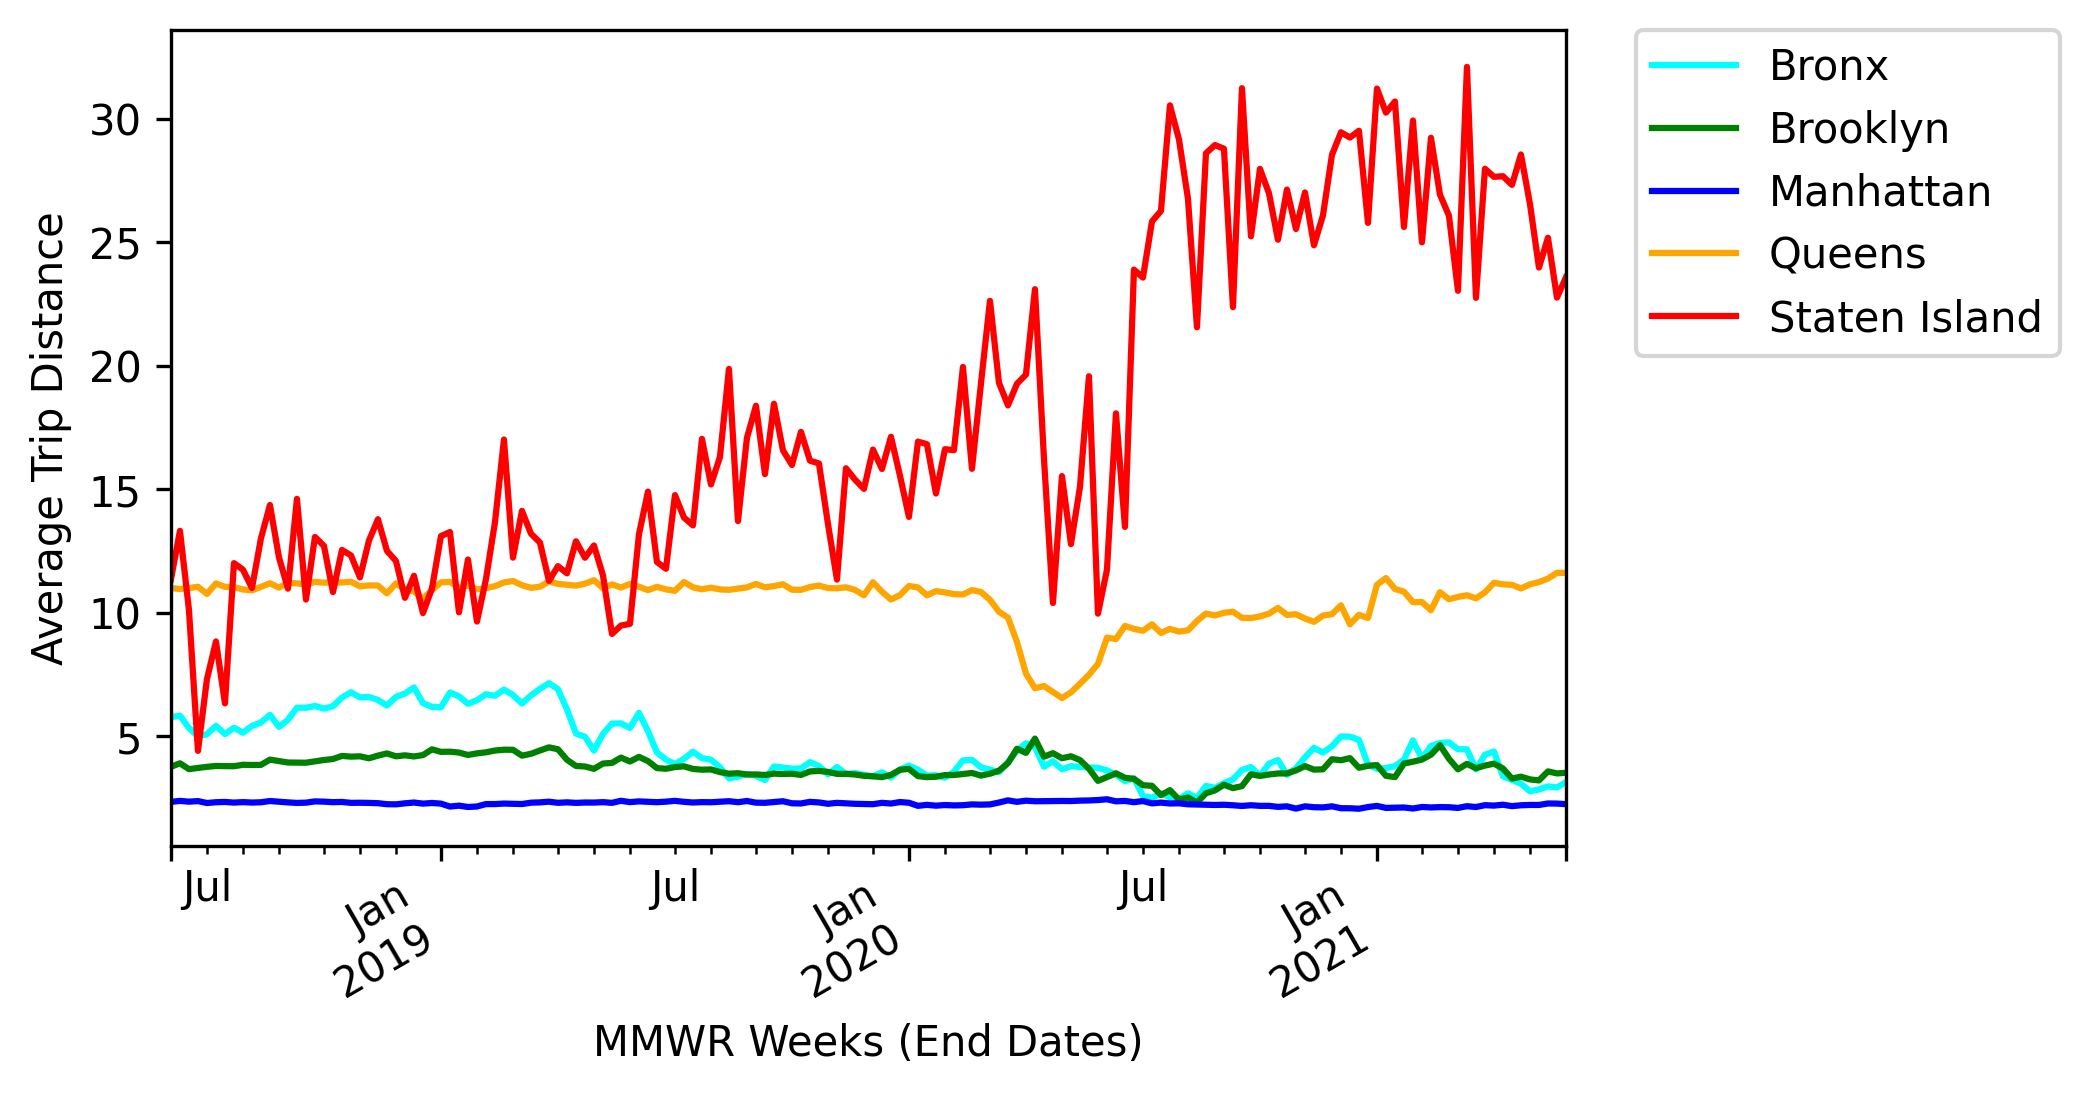
\includegraphics[width=0.5\textwidth]{../plots/time-series-Average Trip Distance-vs-MMWR Weeks (End Dates)-by-pu_borough.png}
        % 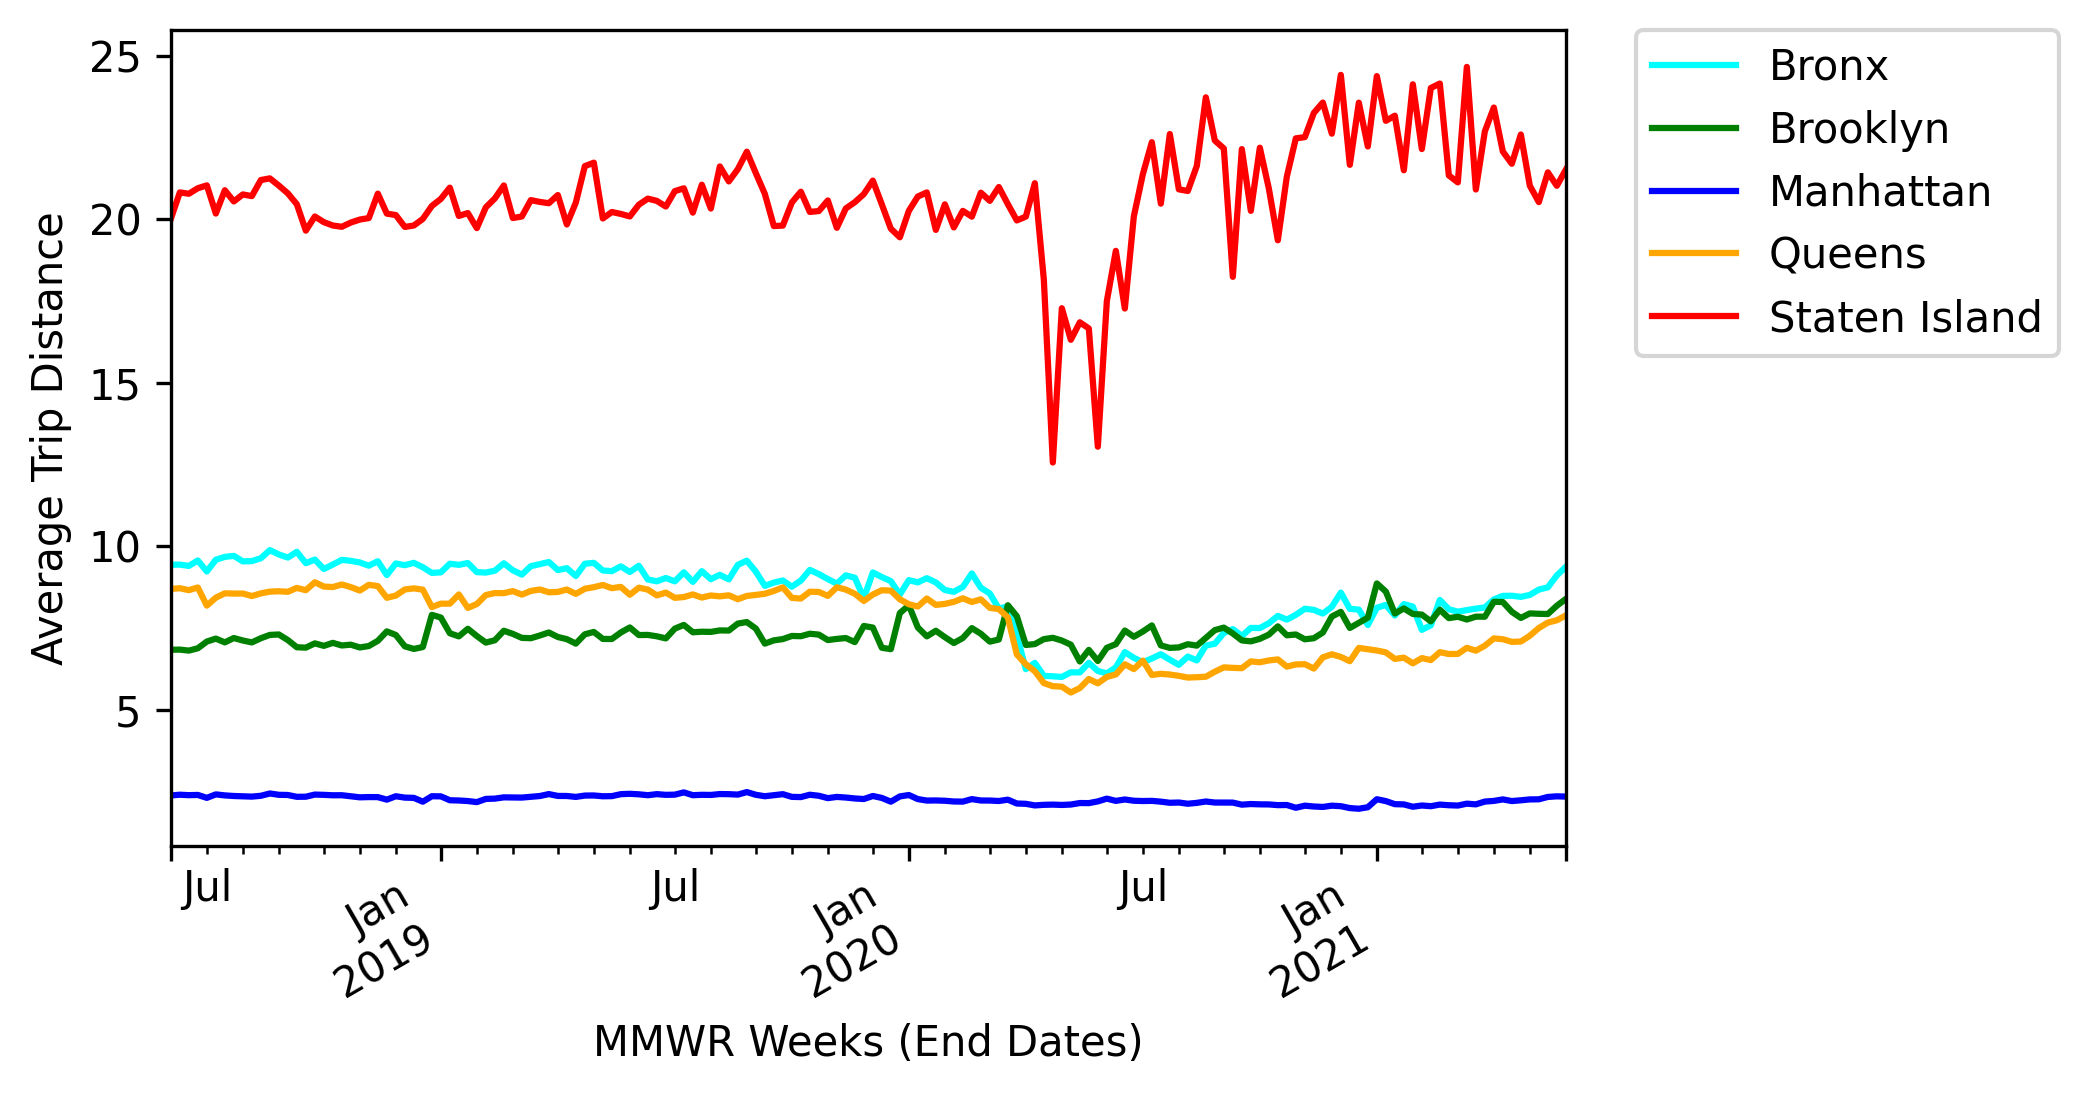
\includegraphics[width=0.45\textwidth]{../plots/time-series-Average Trip Distance-vs-MMWR Weeks (End Dates)-by-do_borough.png}
        % this ensures your figures are centered where possible
        \centering
        \caption{How average trip distances per week per pickup borough vary over time.} % refer to this image as (Figure 1)
        \label{fig:ts-dist-weeks}
    \end{figure}

    \begin{figure}[H]
        % change the scale multiplier to make the figures smaller or larger
        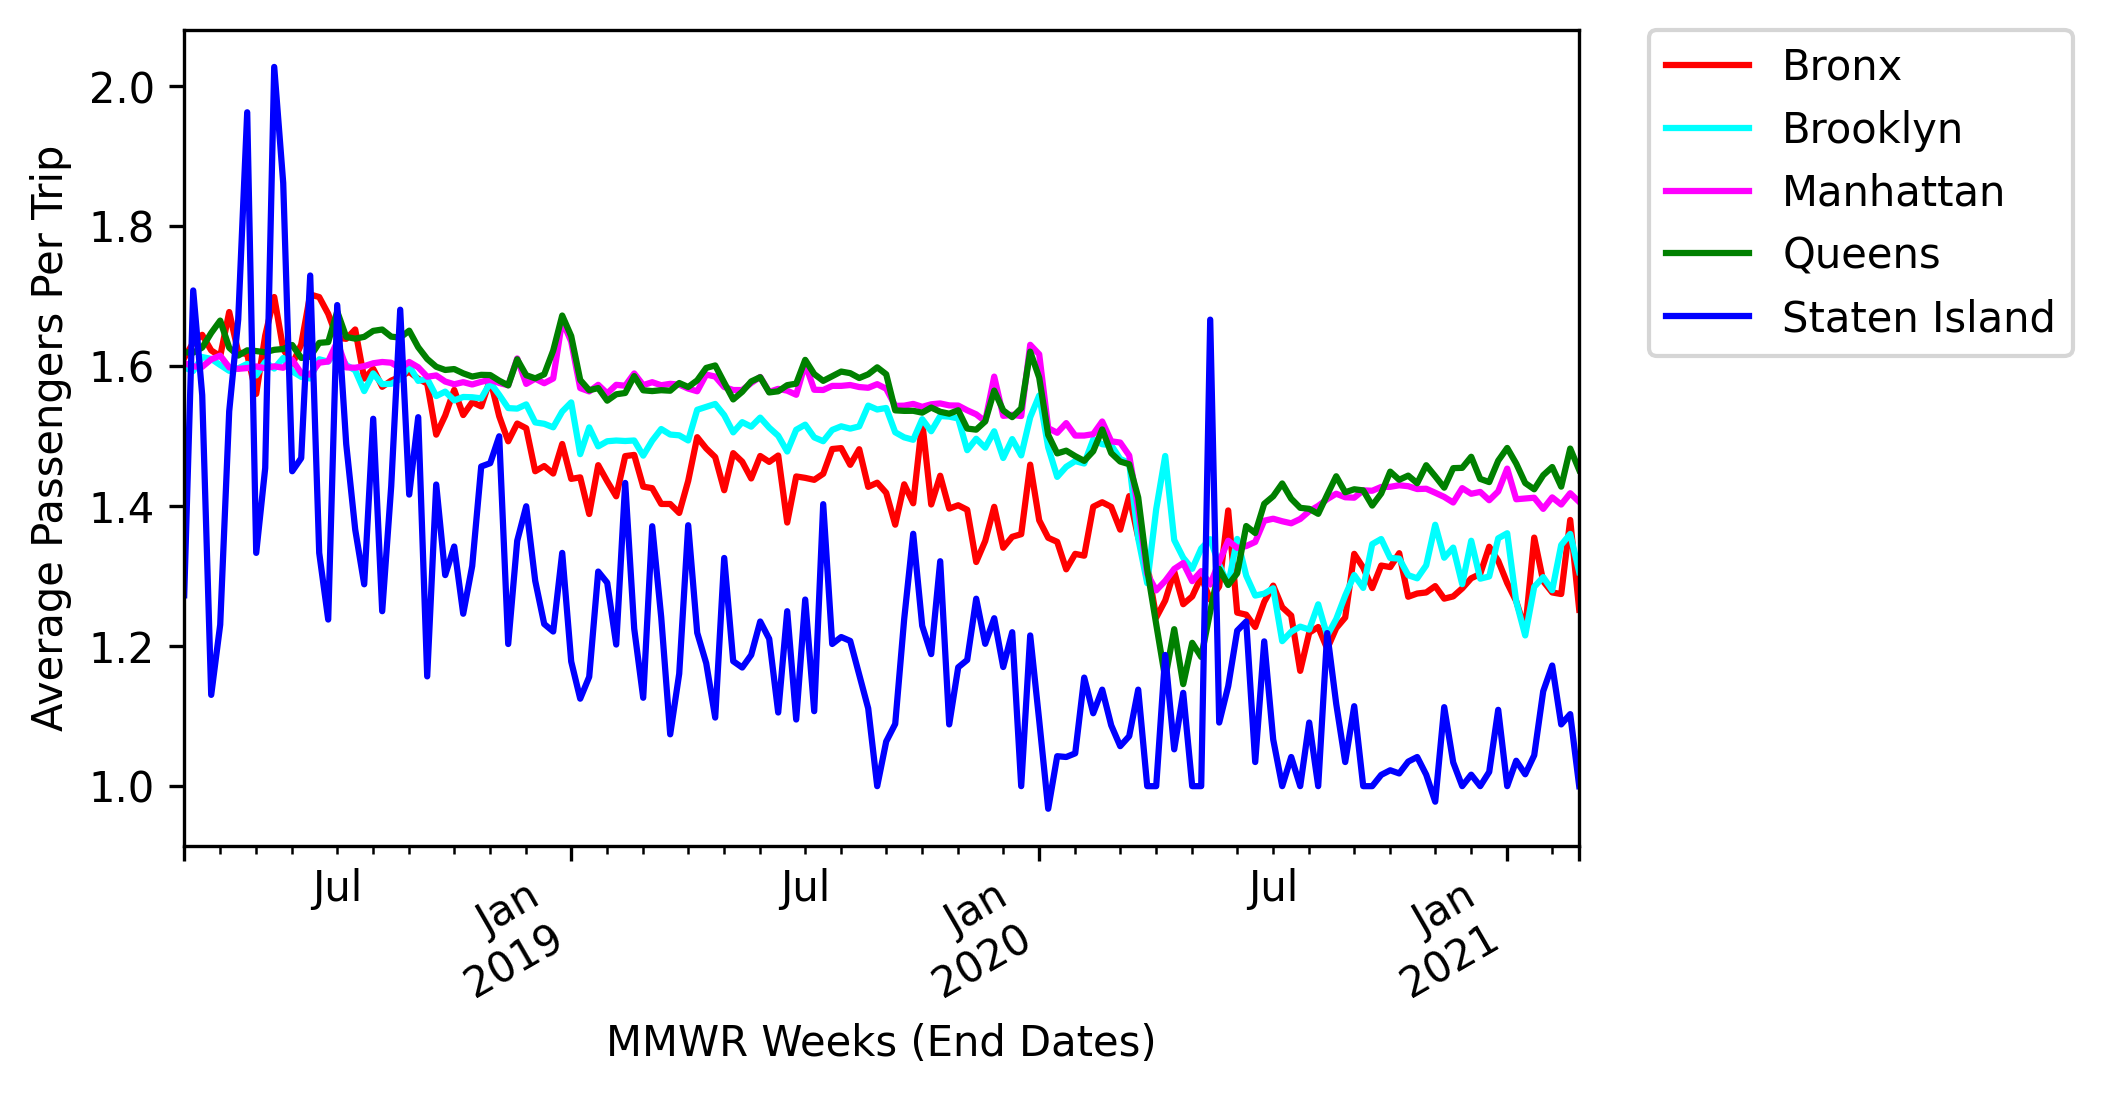
\includegraphics[width=0.5\textwidth]{../plots/time-series-Average Passengers Per Trip-vs-MMWR Weeks (End Dates)-by-pu_borough.png}
        % 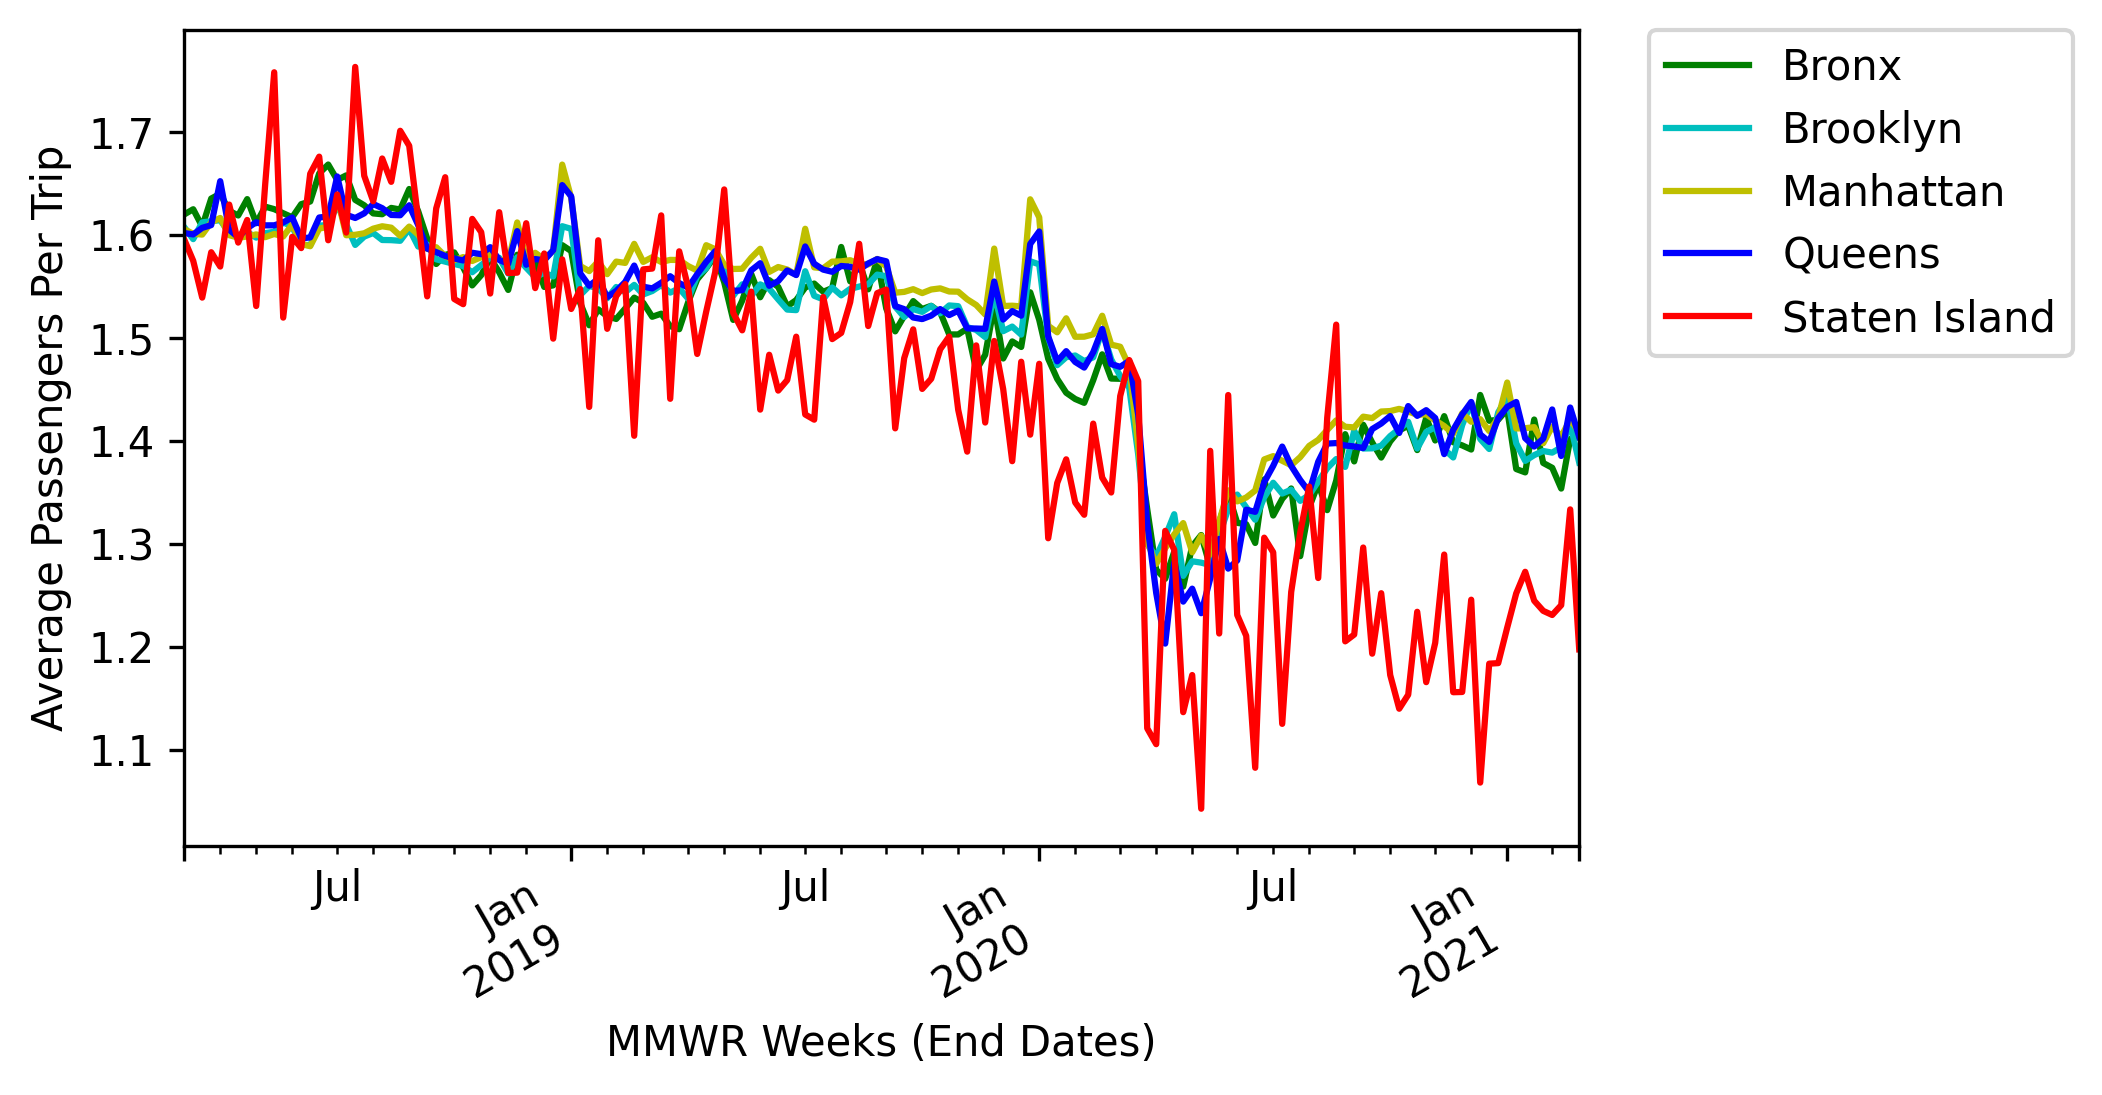
\includegraphics[width=0.45\textwidth]{../plots/time-series-Average Passengers Per Trip-vs-MMWR Weeks (End Dates)-by-do_borough.png}
        % this ensures your figures are centered where possible
        \centering
        \caption{How average passenger counts per week per pickup borough vary over time.} % refer to this image as (Figure 1)
        \label{fig:ts-pass-count-weeks}
    \end{figure}
\end{multicols}

% \begin{figure}[h]
%     % change the scale multiplier to make the figures smaller or larger
%     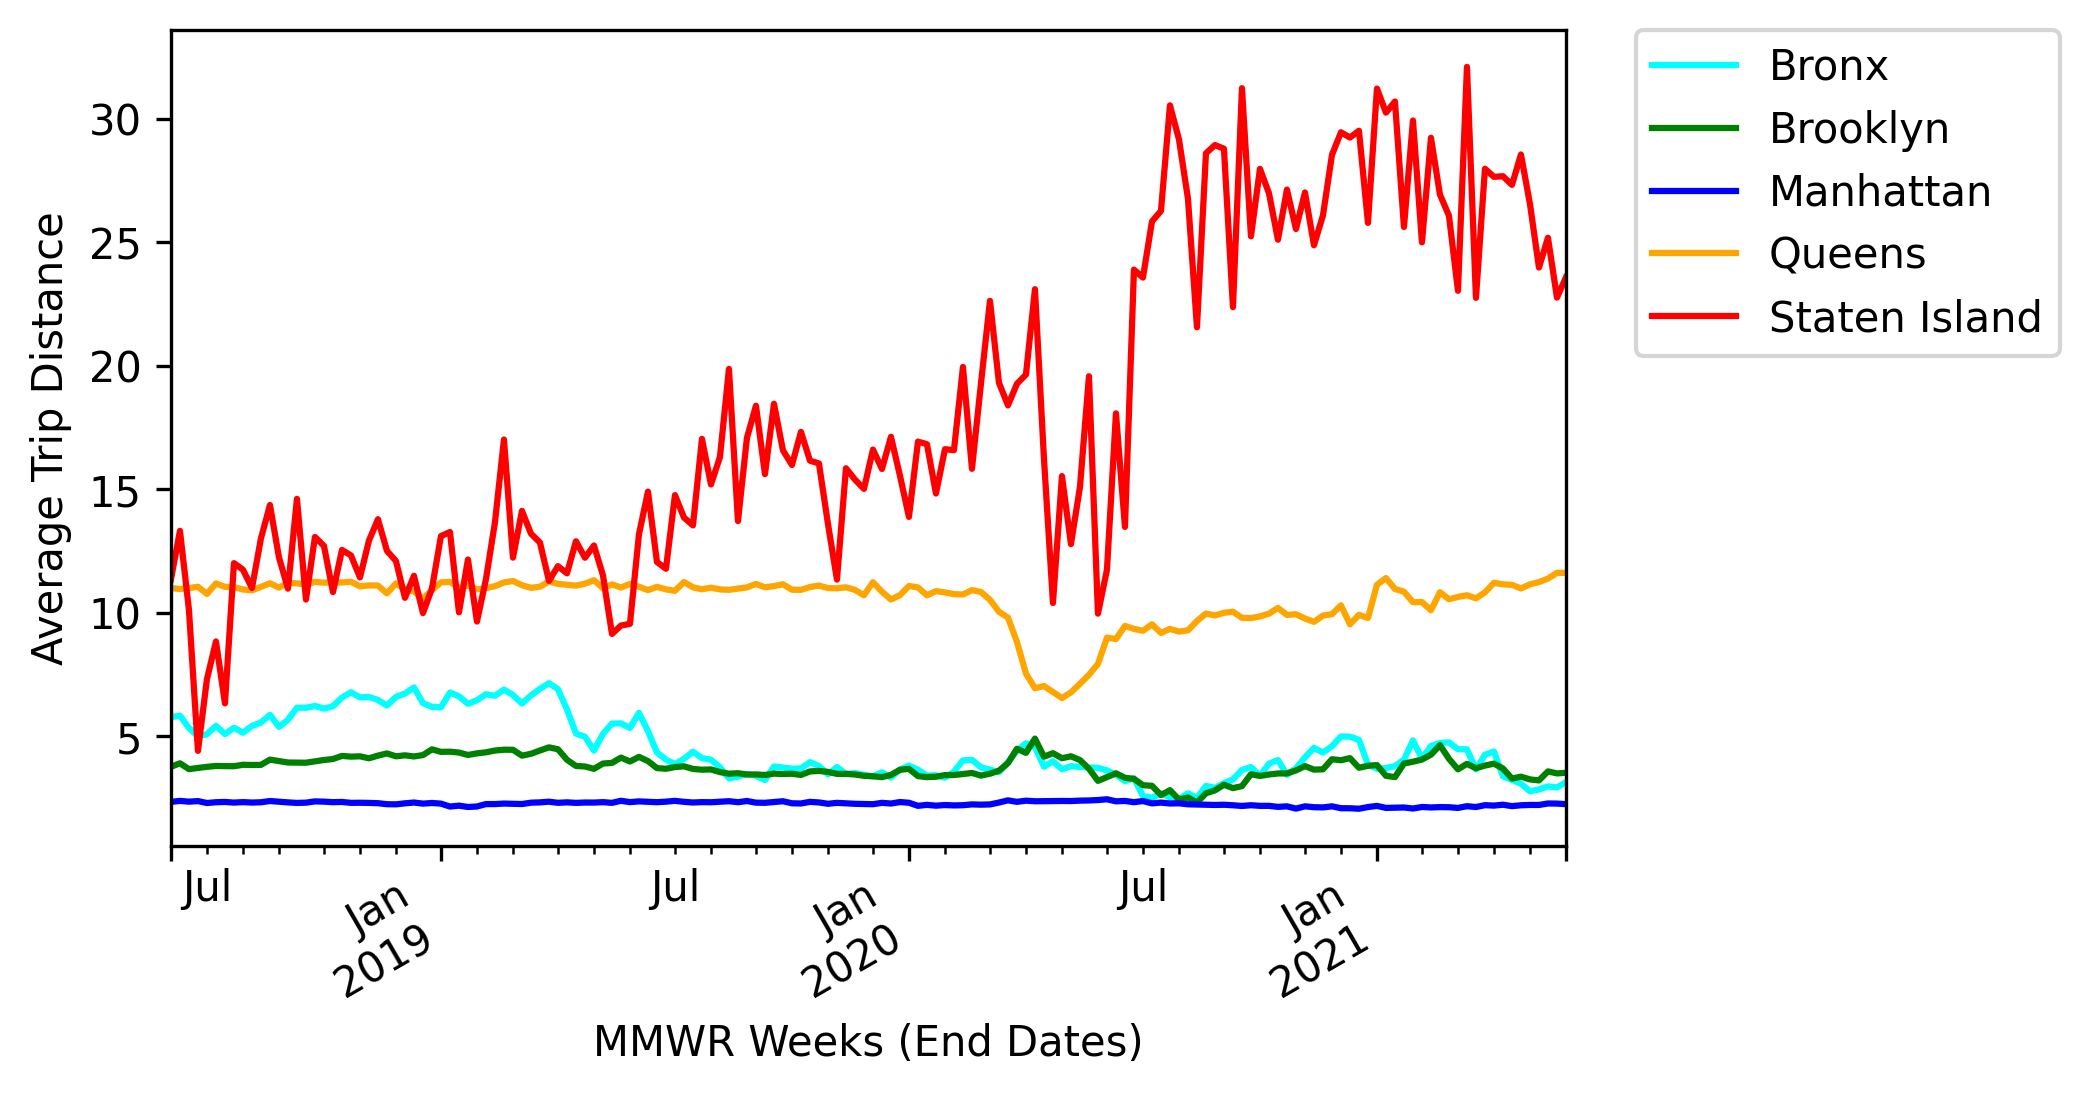
\includegraphics[width=0.45\textwidth]{../plots/time-series-Average Trip Distance-vs-MMWR Weeks (End Dates)-by-pu_borough.png}
%     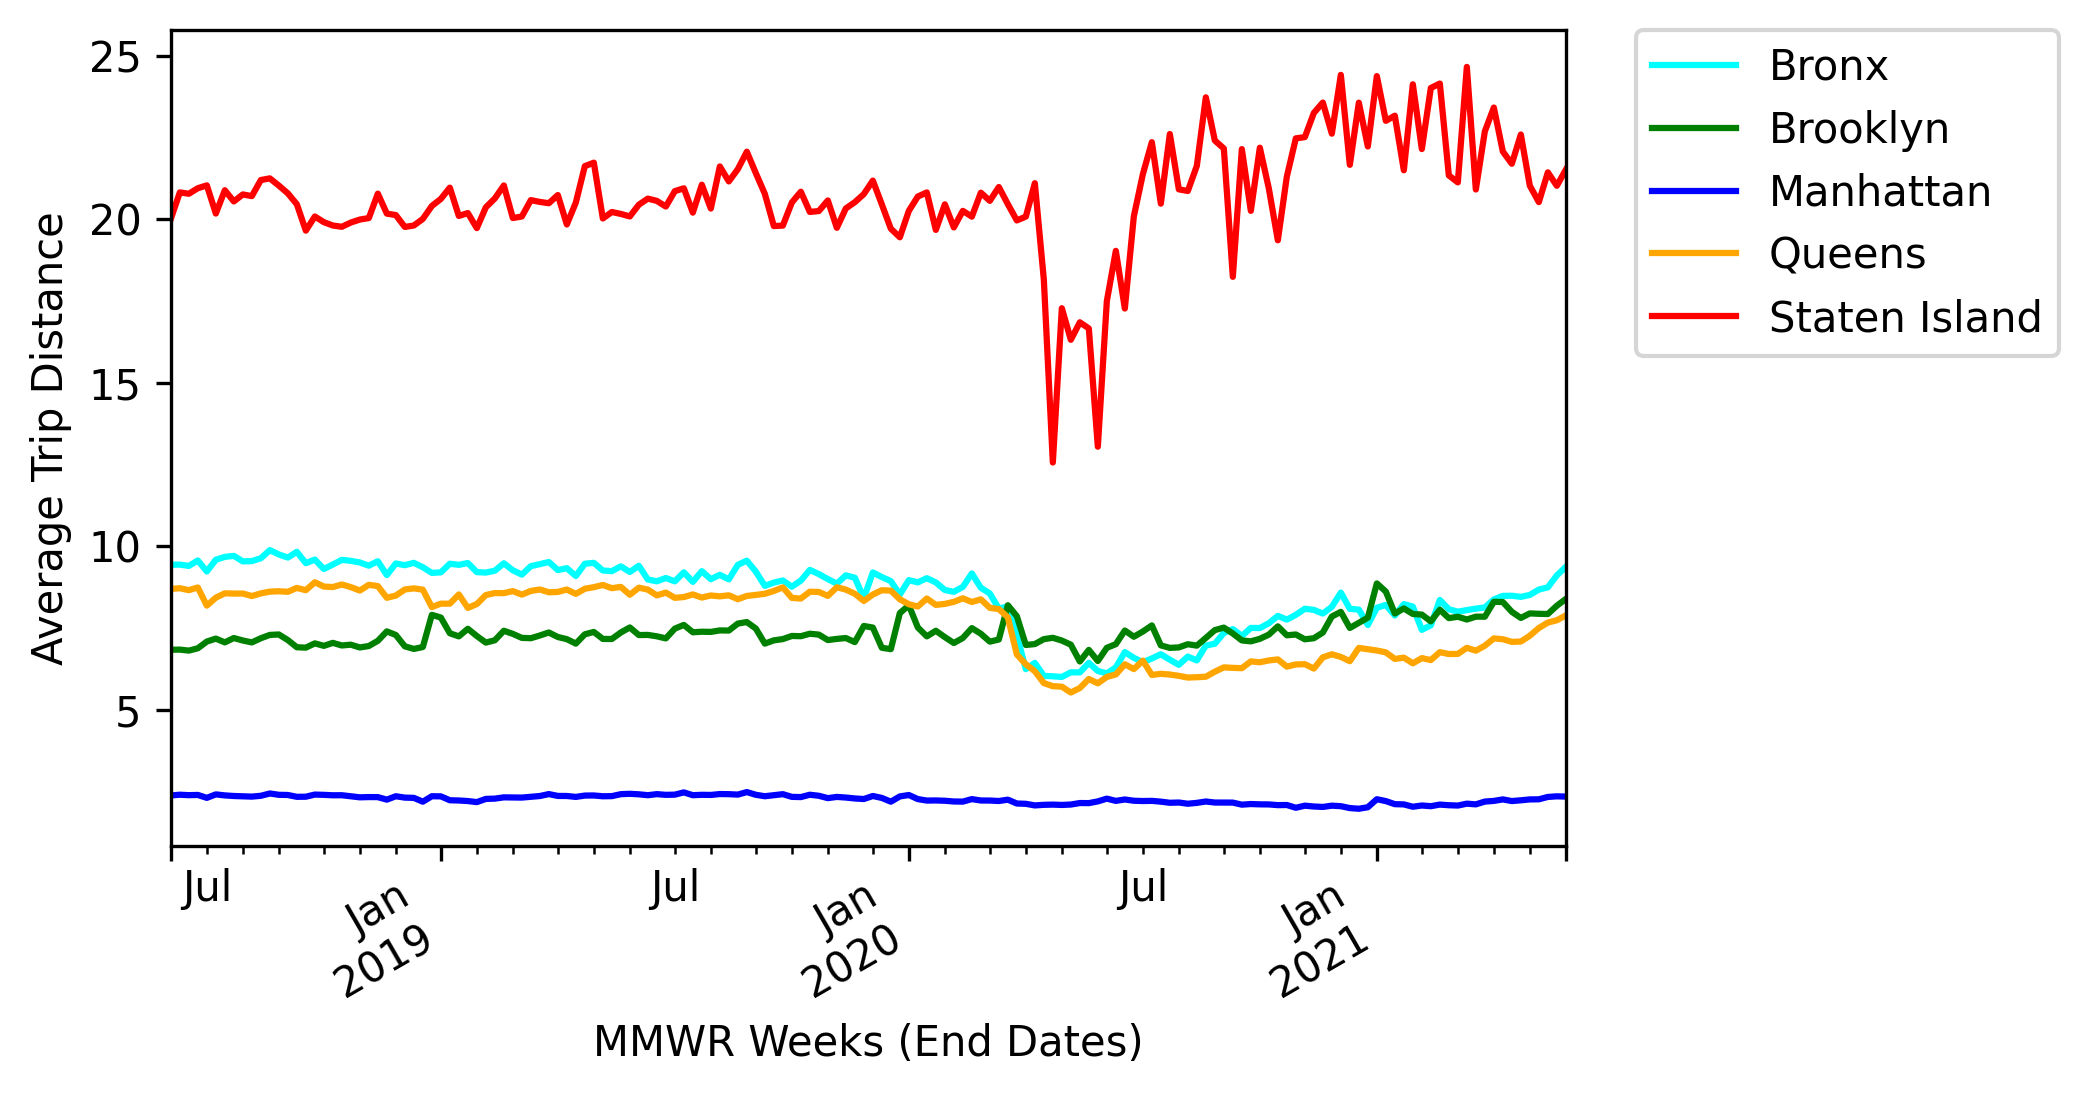
\includegraphics[width=0.45\textwidth]{../plots/time-series-Average Trip Distance-vs-MMWR Weeks (End Dates)-by-do_borough.png}
%     % this ensures your figures are centered where possible
%     \centering
%     \caption{How average trip distances per week per pickup (left) and dropoff (right) borough vary over time.} % refer to this image as (Figure 1)
%     \label{fig:ts-dist-weeks}
% \end{figure}

This uptick in travel distance is likely caused by reduced usage of the Staten Island ferry and the reduced schedule during the pandemic \cite{dot2020}.
If this is the case, then Figure~\ref{fig:ts-dist-weeks} suggests that people travelling to and from Staten Island rely on taxis to be safer and ontime over the ferry service.
The trip distances between boroughs are generally not very homoegeneous. 
A likely reason for this heterogeneity is the difference in commutes to work, since
many jobs are likely located in Manhattan.

Figure~\ref{fig:ts-pass-count-weeks} shows average trip passenger counts per MMWR week.
According to Figures~\ref{fig:ts-dist-weeks} and \ref{fig:ts-pass-count-weeks}, 
it appears as though passenger counts experience more drastic variation week-on-week.
Such instability may present in a weaker linear model being generated for passenger count.
% \begin{figure}[h]
%     % change the scale multiplier to make the figures smaller or larger
%     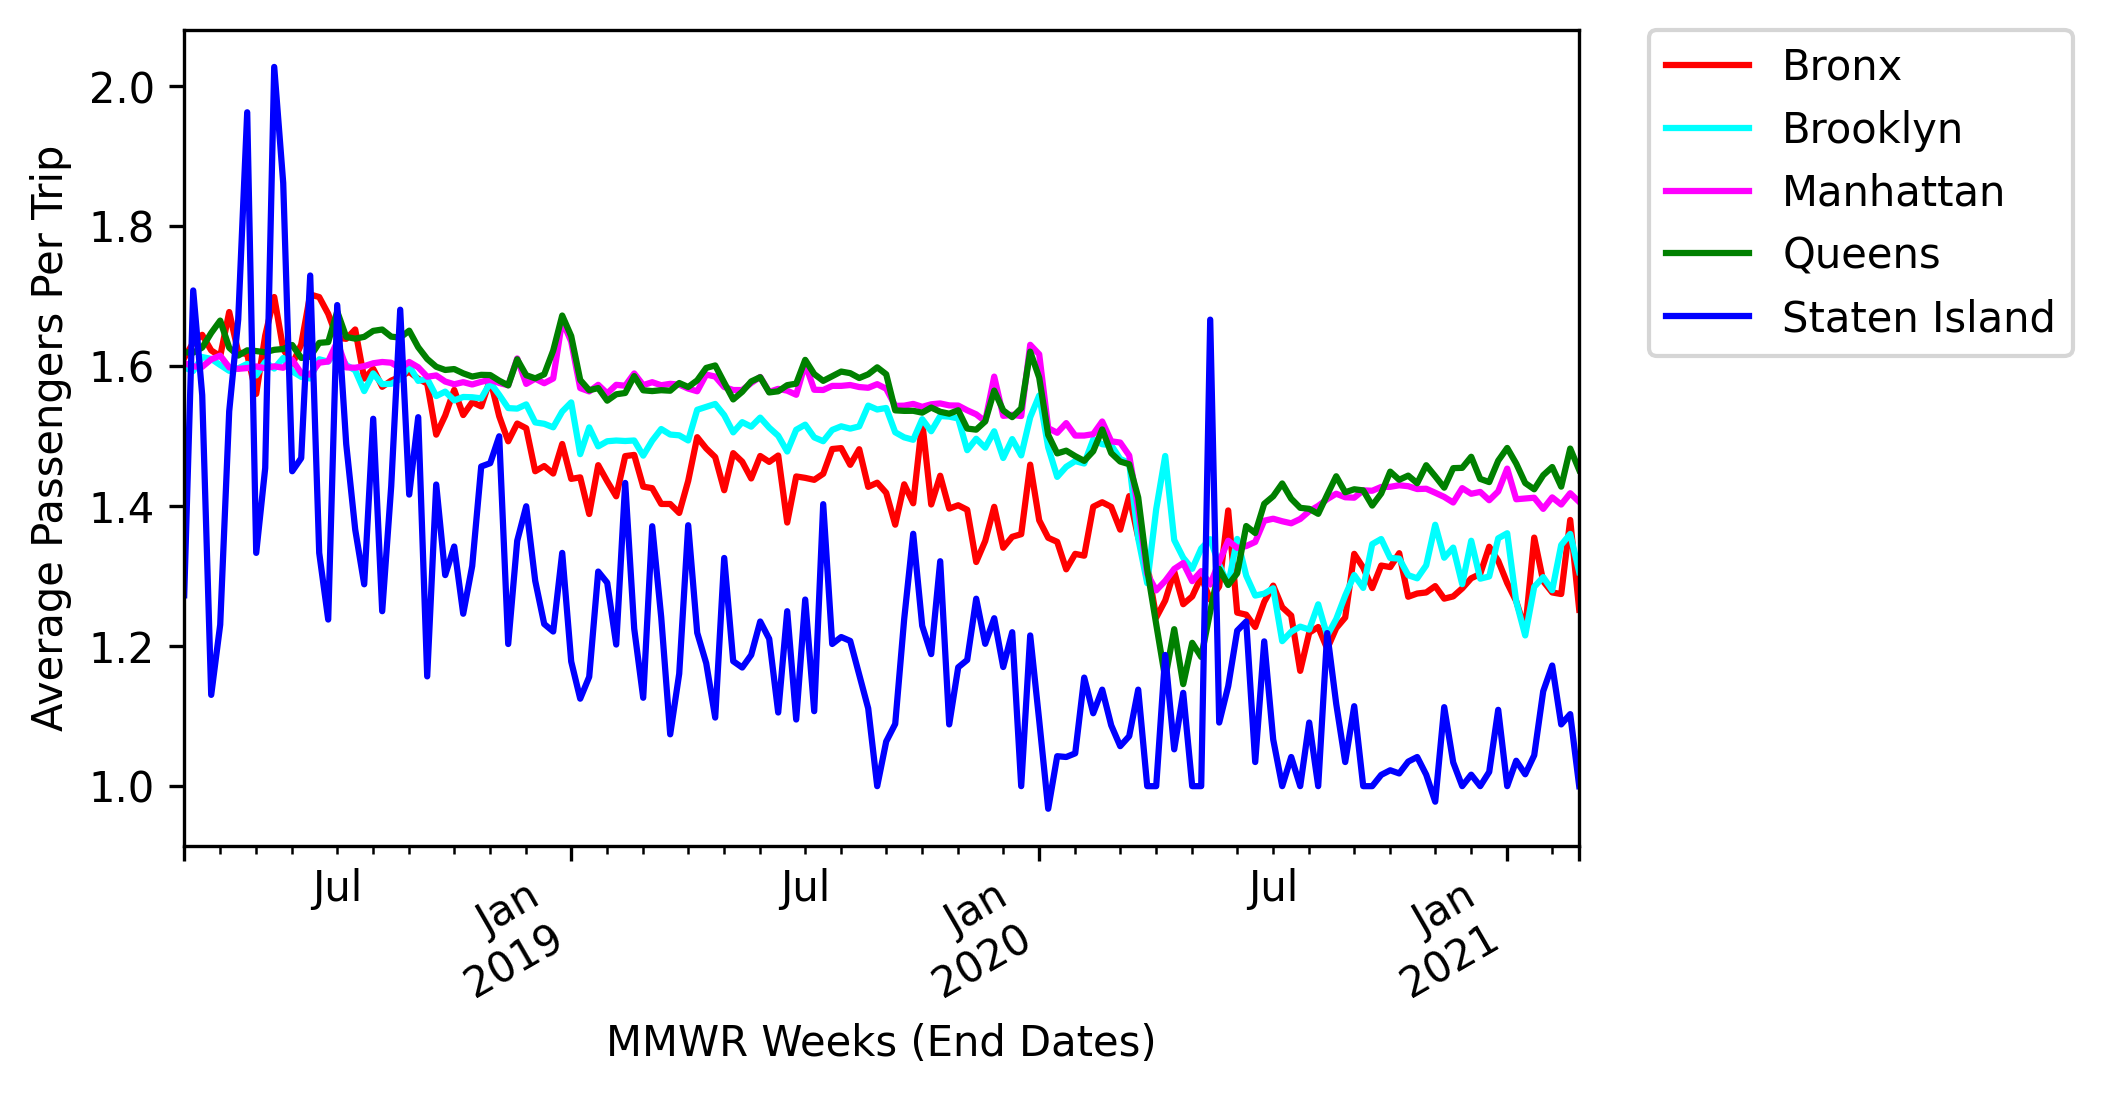
\includegraphics[width=0.45\textwidth]{../plots/time-series-Average Passengers Per Trip-vs-MMWR Weeks (End Dates)-by-pu_borough.png}
%     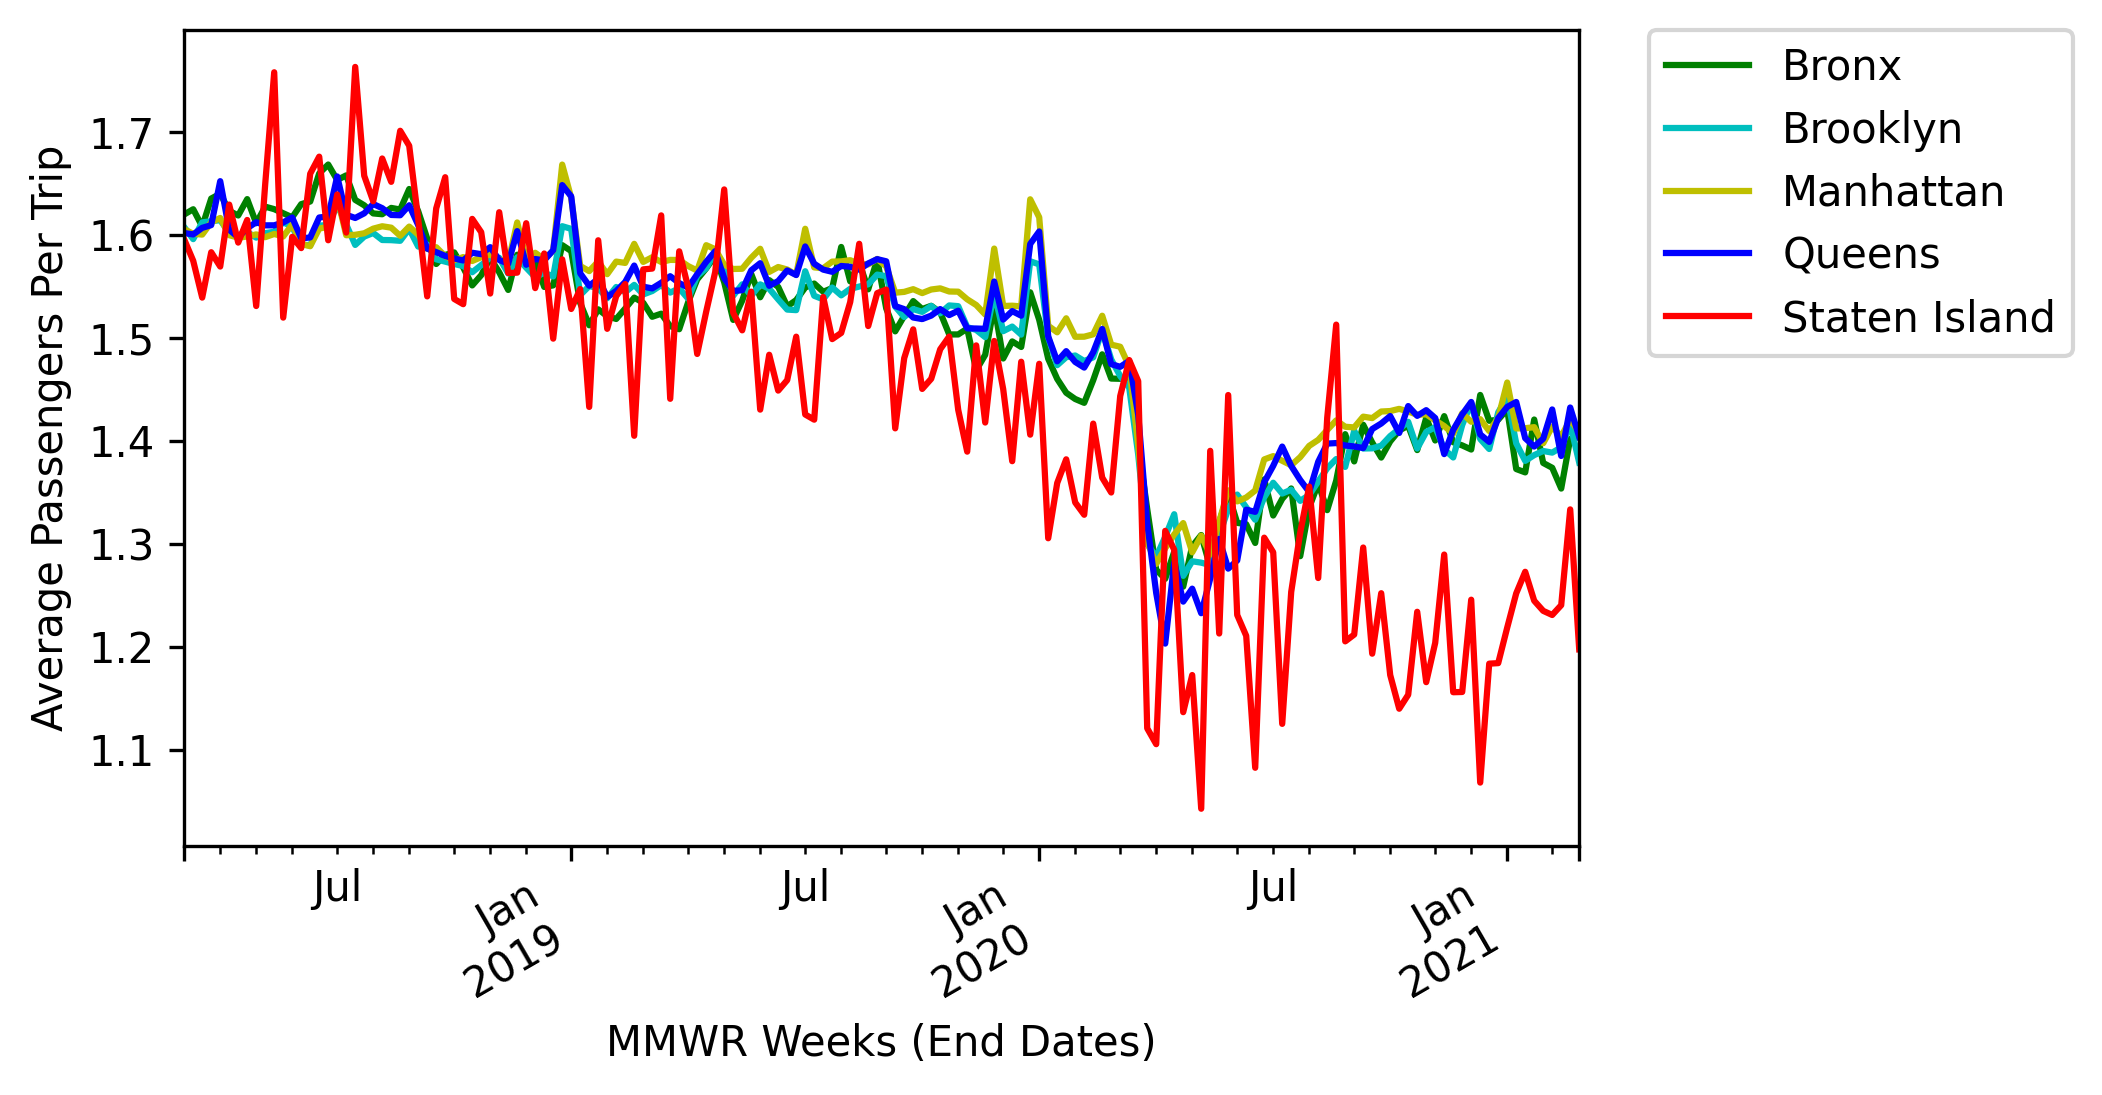
\includegraphics[width=0.45\textwidth]{../plots/time-series-Average Passengers Per Trip-vs-MMWR Weeks (End Dates)-by-do_borough.png}
%     % this ensures your figures are centered where possible
%     \centering
%     \caption{How average passenger count per week per pickup (left) and dropoff (right) borough vary over time.} % refer to this image as (Figure 1)
%     \label{fig:ts-pass-count-weeks}
% \end{figure}


% \begin{figure}[H]
%     % change the scale multiplier to make the figures smaller or larger
%     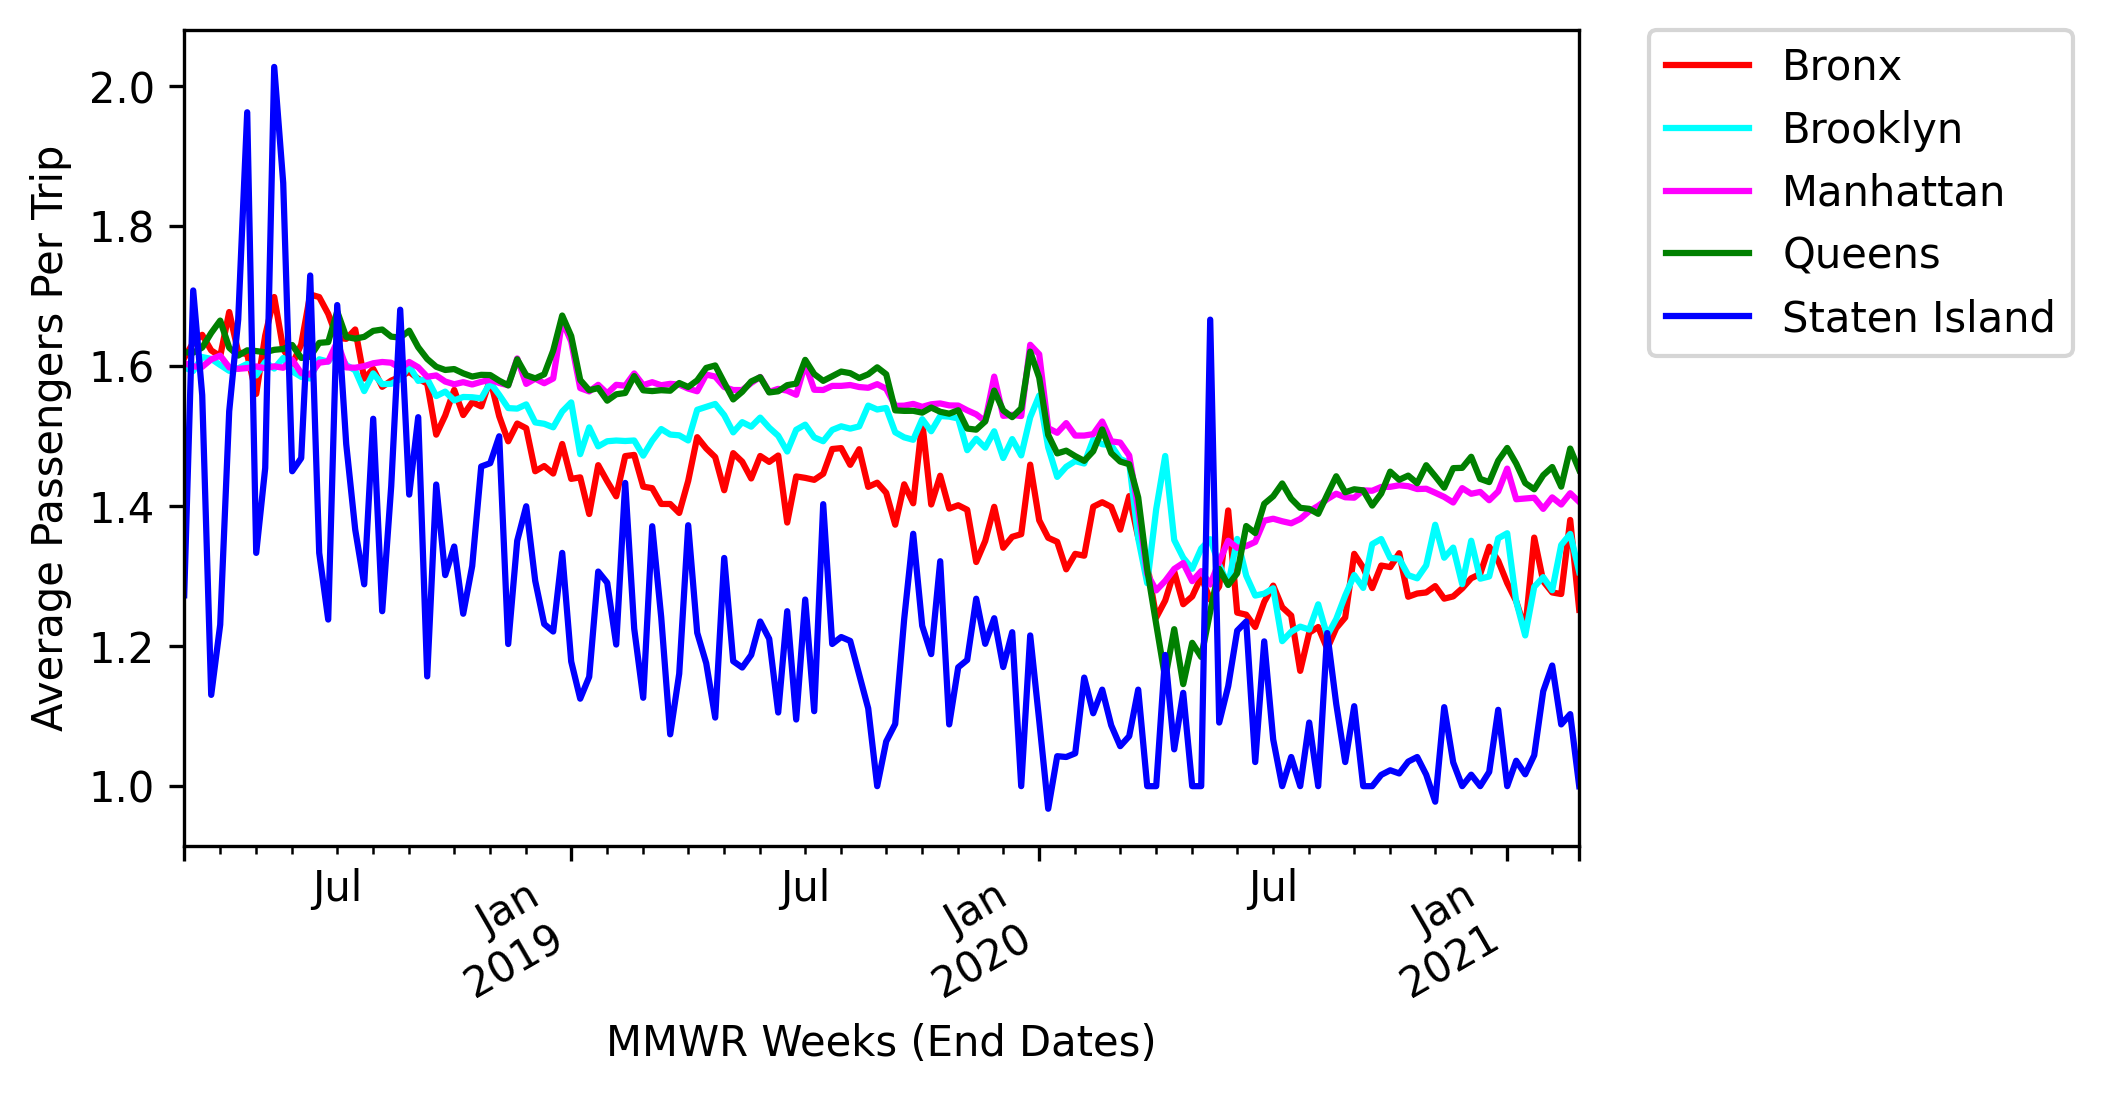
\includegraphics[width=0.5\textwidth]{../plots/time-series-Average Passengers Per Trip-vs-MMWR Weeks (End Dates)-by-pu_borough.png}
%     % 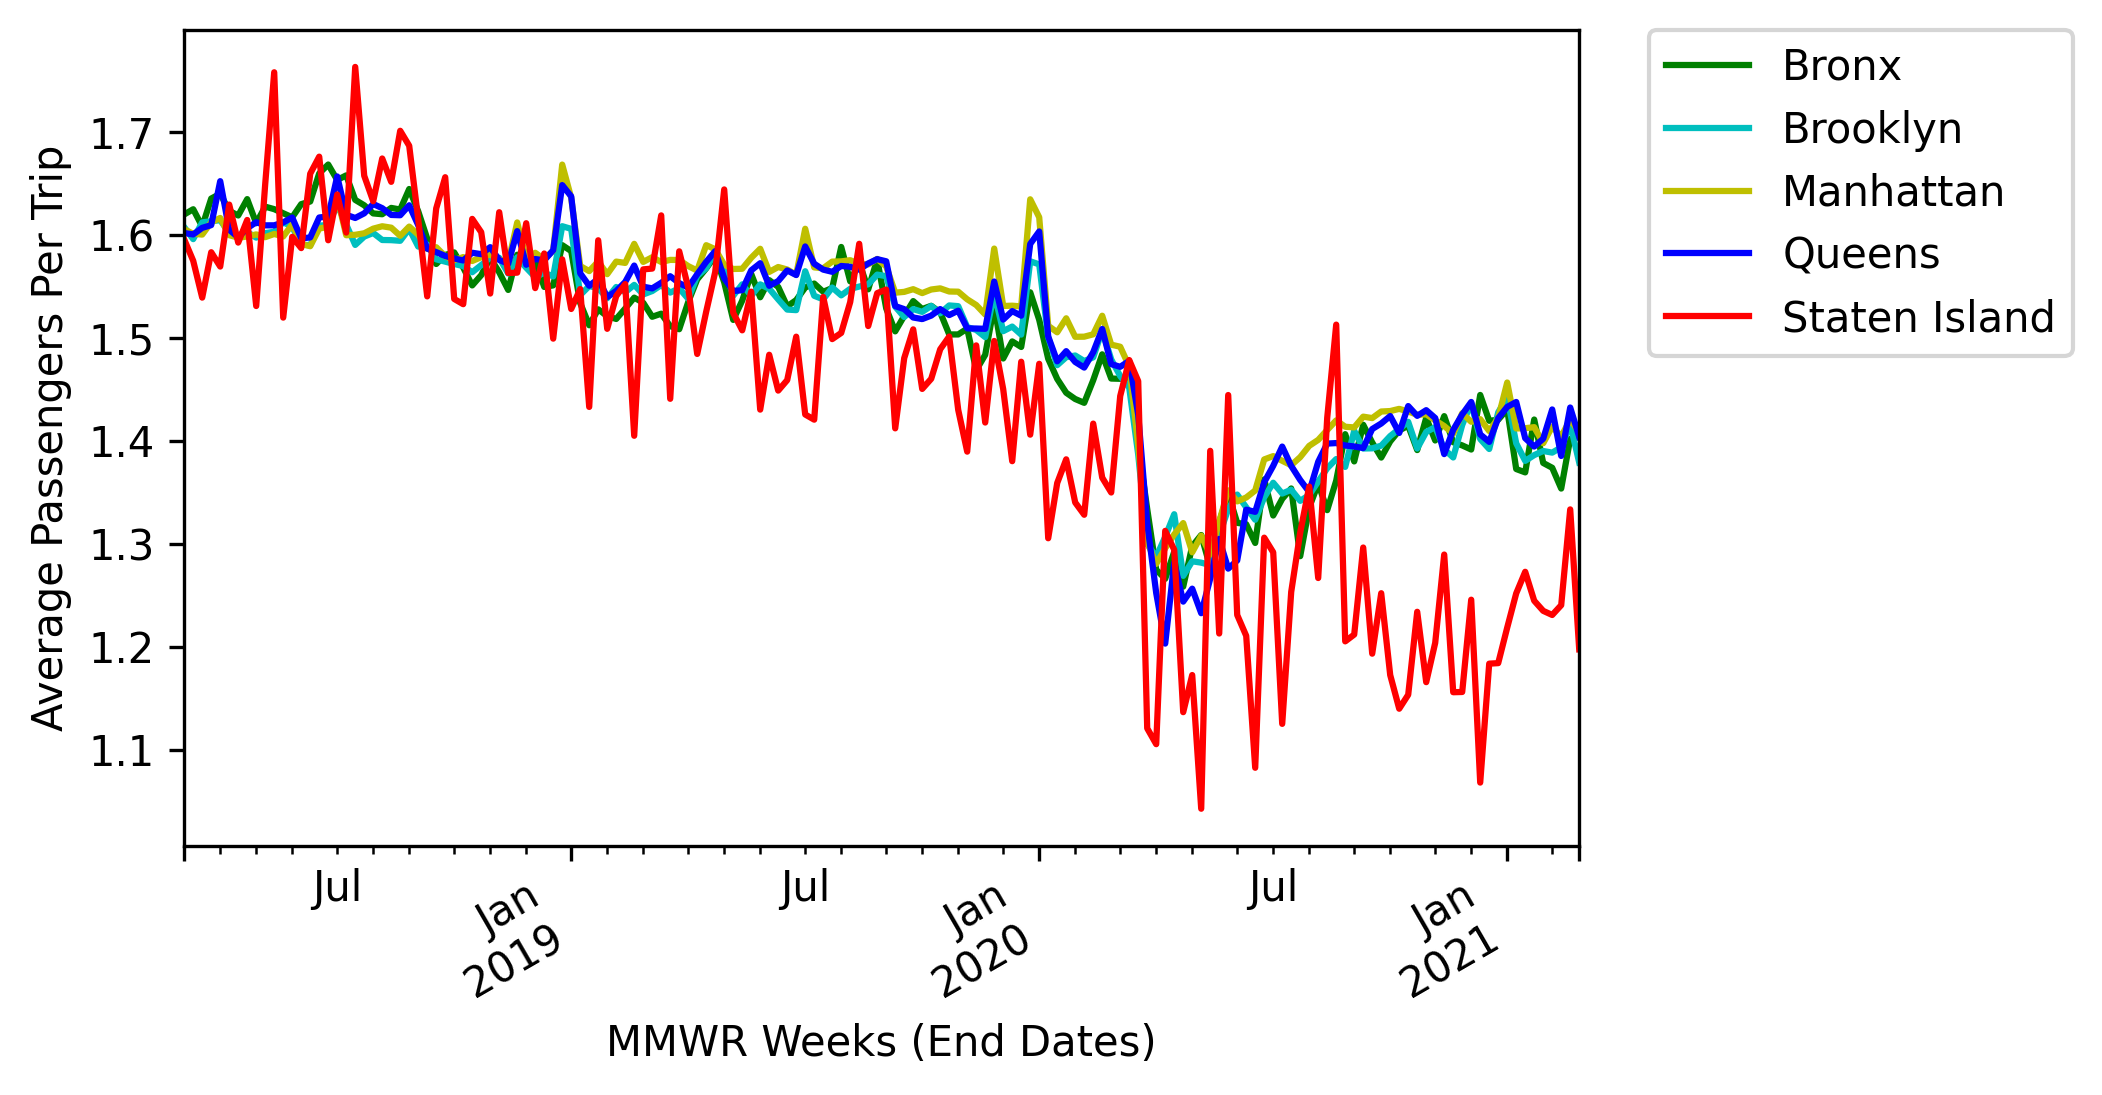
\includegraphics[width=0.45\textwidth]{../plots/time-series-Average Passengers Per Trip-vs-MMWR Weeks (End Dates)-by-do_borough.png}
%     % this ensures your figures are centered where possible
%     \centering
%     \caption{How average passenger counts per week per pickup borough vary over time.} % refer to this image as (Figure 1)
%     \label{fig:ts-pass-count-weeks}
% \end{figure}


The greatest instability in passenger counts appears to come from trips going to or from Staten Island,
while travel to or from other boroughs appears more stable and similar week-on-week. 
This may also come as a result of Staten Island's separation from the other boroughs,
however a true cause and effect relationship on this phenomenon would require a properly designed experiment to confirm.

\textbf{Geospatial Visualisation:}
While time series plots display variation in average trip distance over time, 
they do not clearly convey the meaning of these differences.
Figures~\ref{map:overall}, \ref{map:covid}, and \ref{map:flu} compares the average trip radius overall, 
the average trip radius for the week with maximum COVID-19 cases per capita, 
and the week with maximum Influenza cases per capita per pickup borough.


\begin{figure}[H]

    % this ensures your figures are centered where possible
    \centering

    % change the scale multiplier to make the figures smaller or larger
    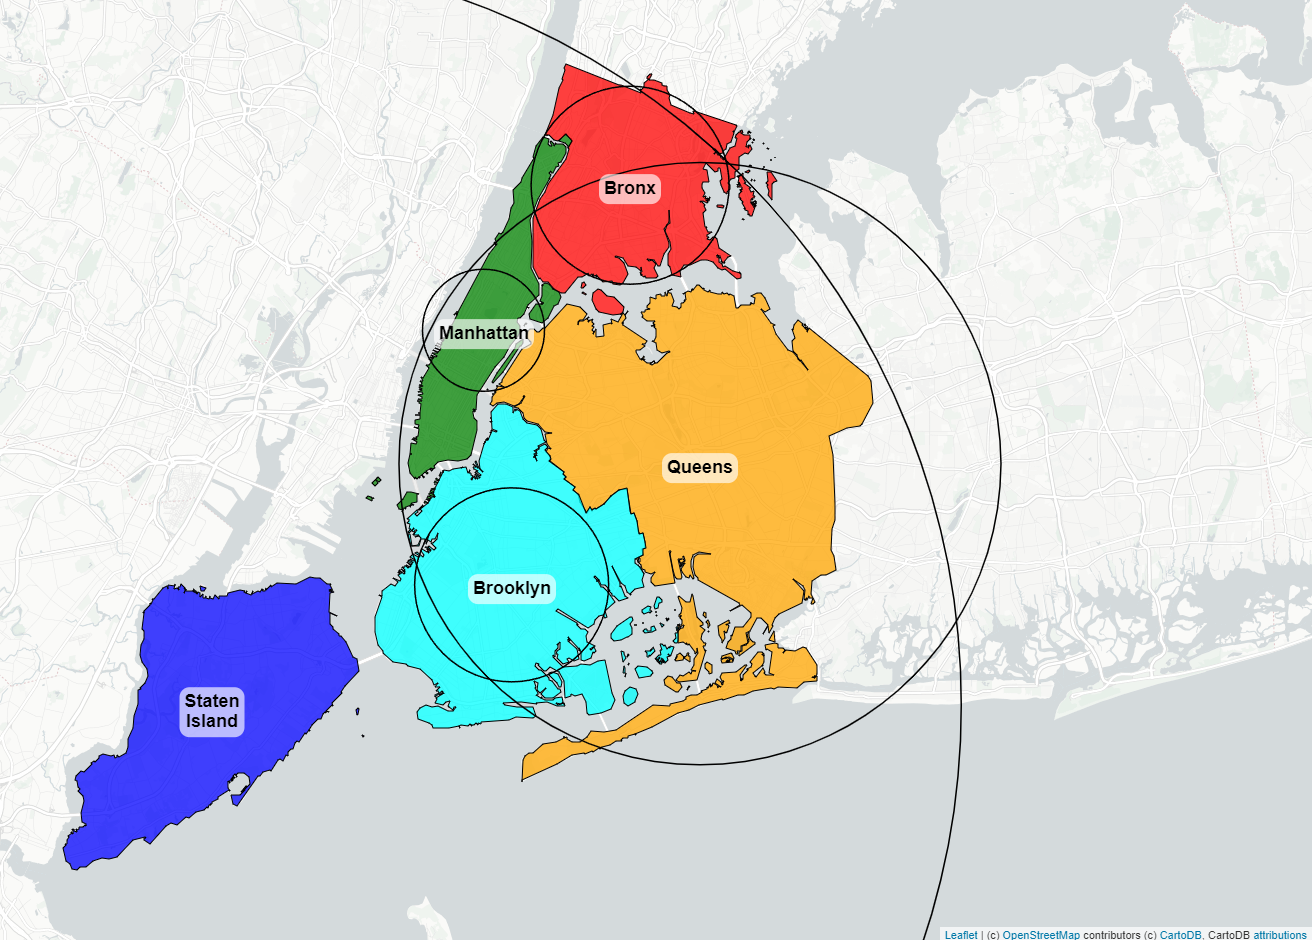
\includegraphics[width=0.45\textwidth]{../plots/map-avg-trip-distance-overall-pu_borough-MODIFIED.png}

    \caption{Map of average trip distance over Timeline 2.} 
    % refer to this image as (Figure 1)
    \label{map:overall}
\end{figure}

% \pagebreak

\begin{multicols}{2}
    \begin{figure}[H]

        % this ensures your figures are centered where possible
        \centering
    
        % change the scale multiplier to make the figures smaller or larger
        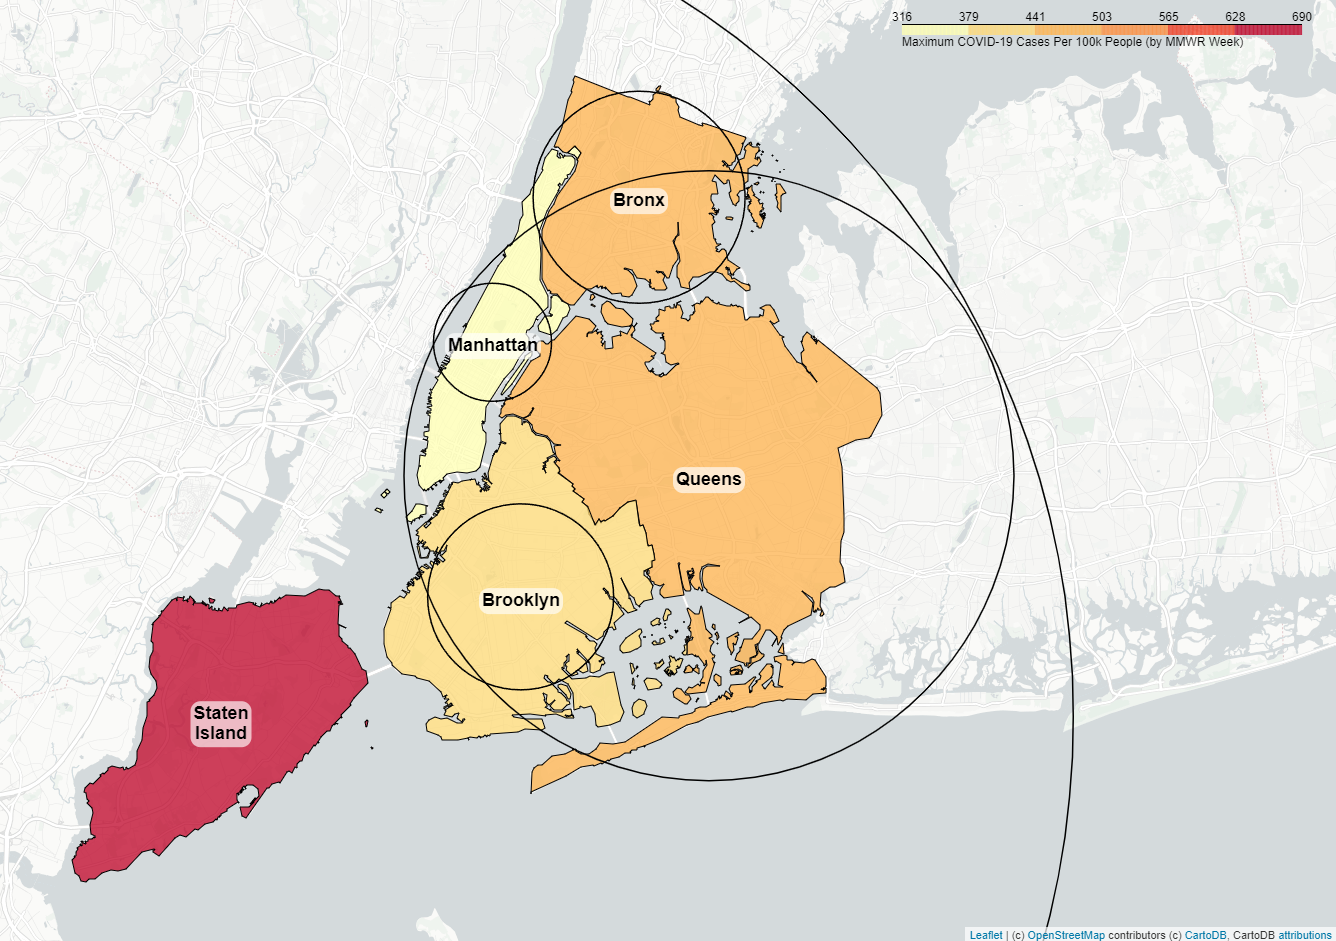
\includegraphics[width=0.45\textwidth]{../plots/map-avg-trip-distance-at-max-covid-by-pu_borough-MODIFIED.png}
    
        \caption{Map of weekly average trip distance following the maximum COVID-19 cases rate over Timeline 2.} % refer to this image as (Figure 1)
        \label{map:covid}
    \end{figure}
    
    \begin{figure}[H]
    
        % this ensures your figures are centered where possible
        \centering
    
        % change the scale multiplier to make the figures smaller or larger
        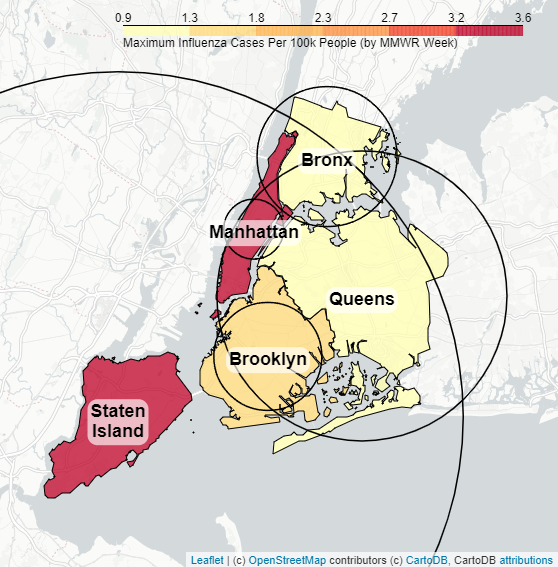
\includegraphics[width=0.45\textwidth]{../plots/map-avg-trip-distance-at-max-flu-by-pu_borough-MODIFIED.png}
    
        \caption{Map of weekly average trip distance following the maximum Influenza cases rate over Timeline 2.} % refer to this image as (Figure 1)
        \label{map:flu}
    \end{figure}    
\end{multicols}

At a first glance, Staten Island appears to experience the most change in trip distance during times of high case rates.
While the initial expectation is that trip distances will decrease following weeks with many virus cases,
the reliance on taxis starting in Staten Island also depends on the type of virus.
Following maximum COVID-19 cases, the average trip radius is wider, 
whereas following maximum Influenza cases, the average trip radius is more constricted.
This suggests that there are different reactions to the prevalence of different viruses.
An alternative explanation is that the Staten Island ferry may have been fully operational when the borough experienced its maximum Influenza case rate.

The other boroughs do not vary as significantly in trip distance.
This may be due to their proximity to each other.
Another contributing factor could be the generally larger populations of these boroughs,
meaning that a larger proportion of people are unlikely to change their taxi usage based on outside factors.


\textbf{Distributions:} 
It is important to note that both average trip distances and passenger counts 
are random variables with different properties, and are therefore modelled using different distributions.
Trip distances are a continuous metric, while passenger counts are discrete, but neither can be negative.
This means that two different forms of linear model are used to model each measure.

\begin{figure}[H]
    % change the scale multiplier to make the figures smaller or larger
    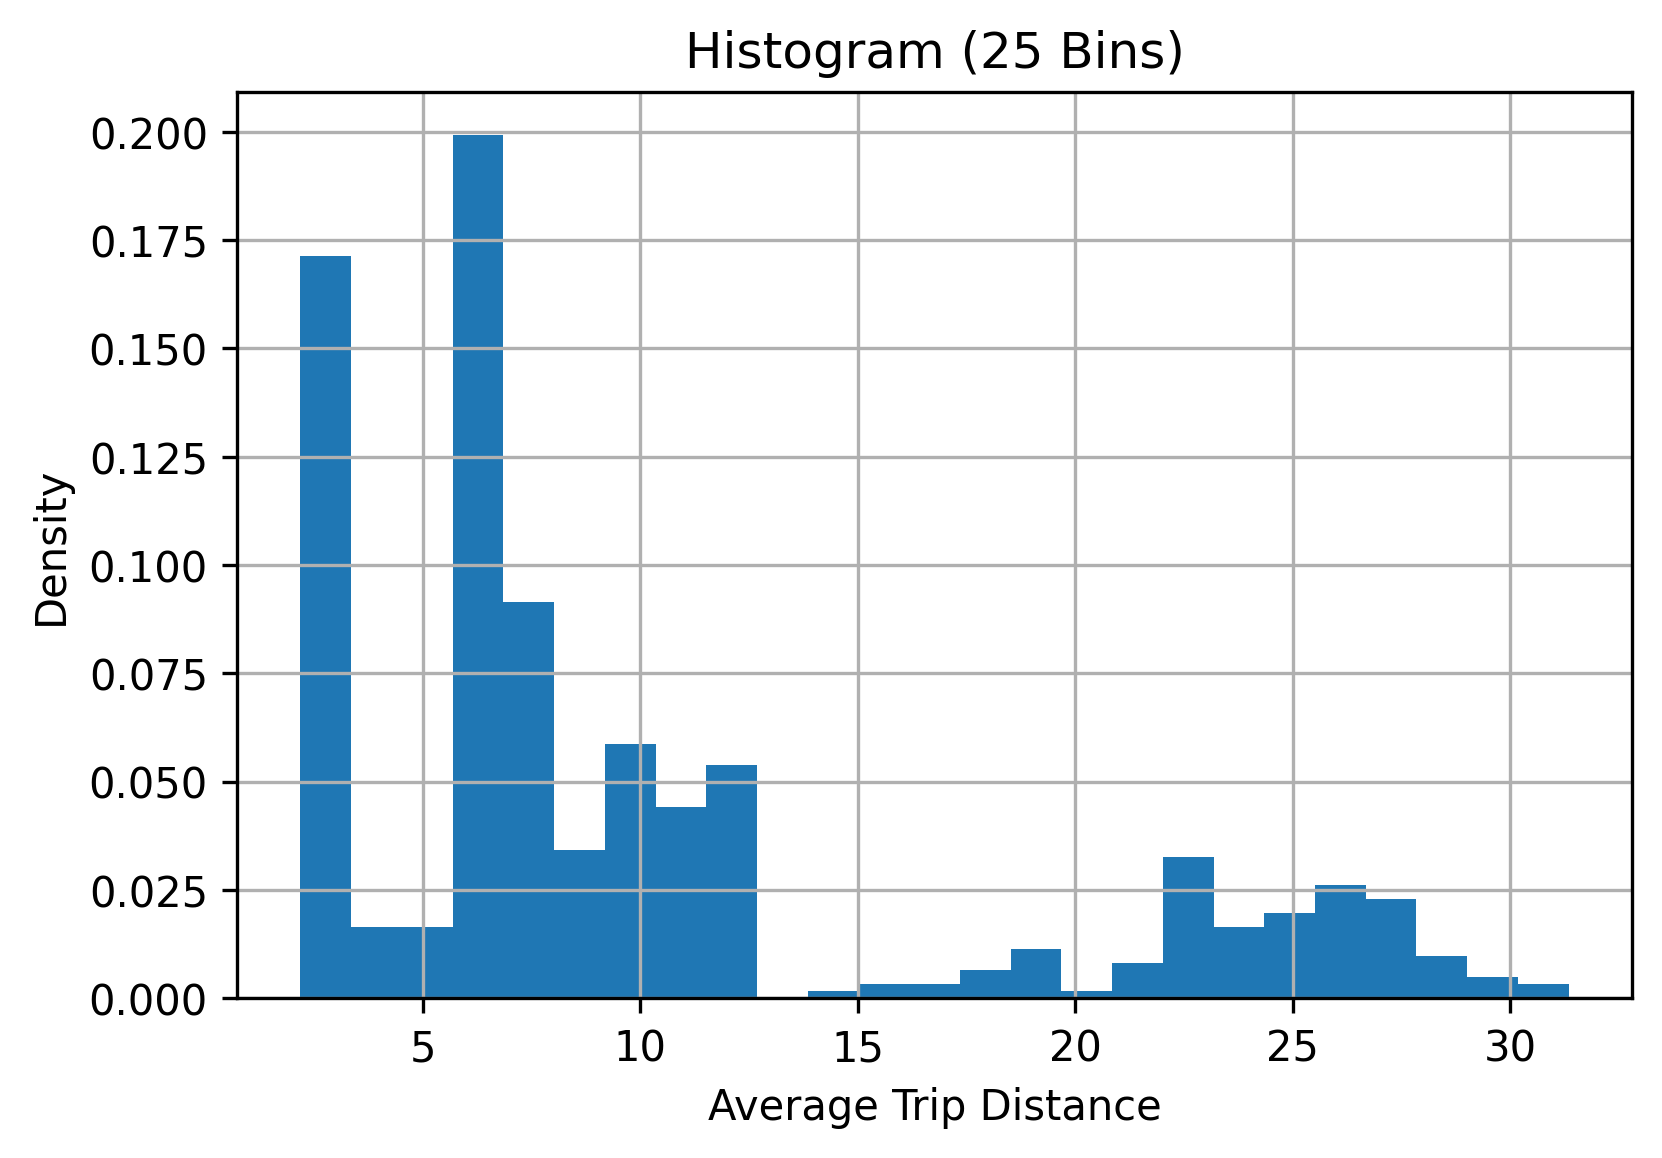
\includegraphics[width=0.40\textwidth]{../plots/histogram-Average Trip Distance-25-bins.png}
    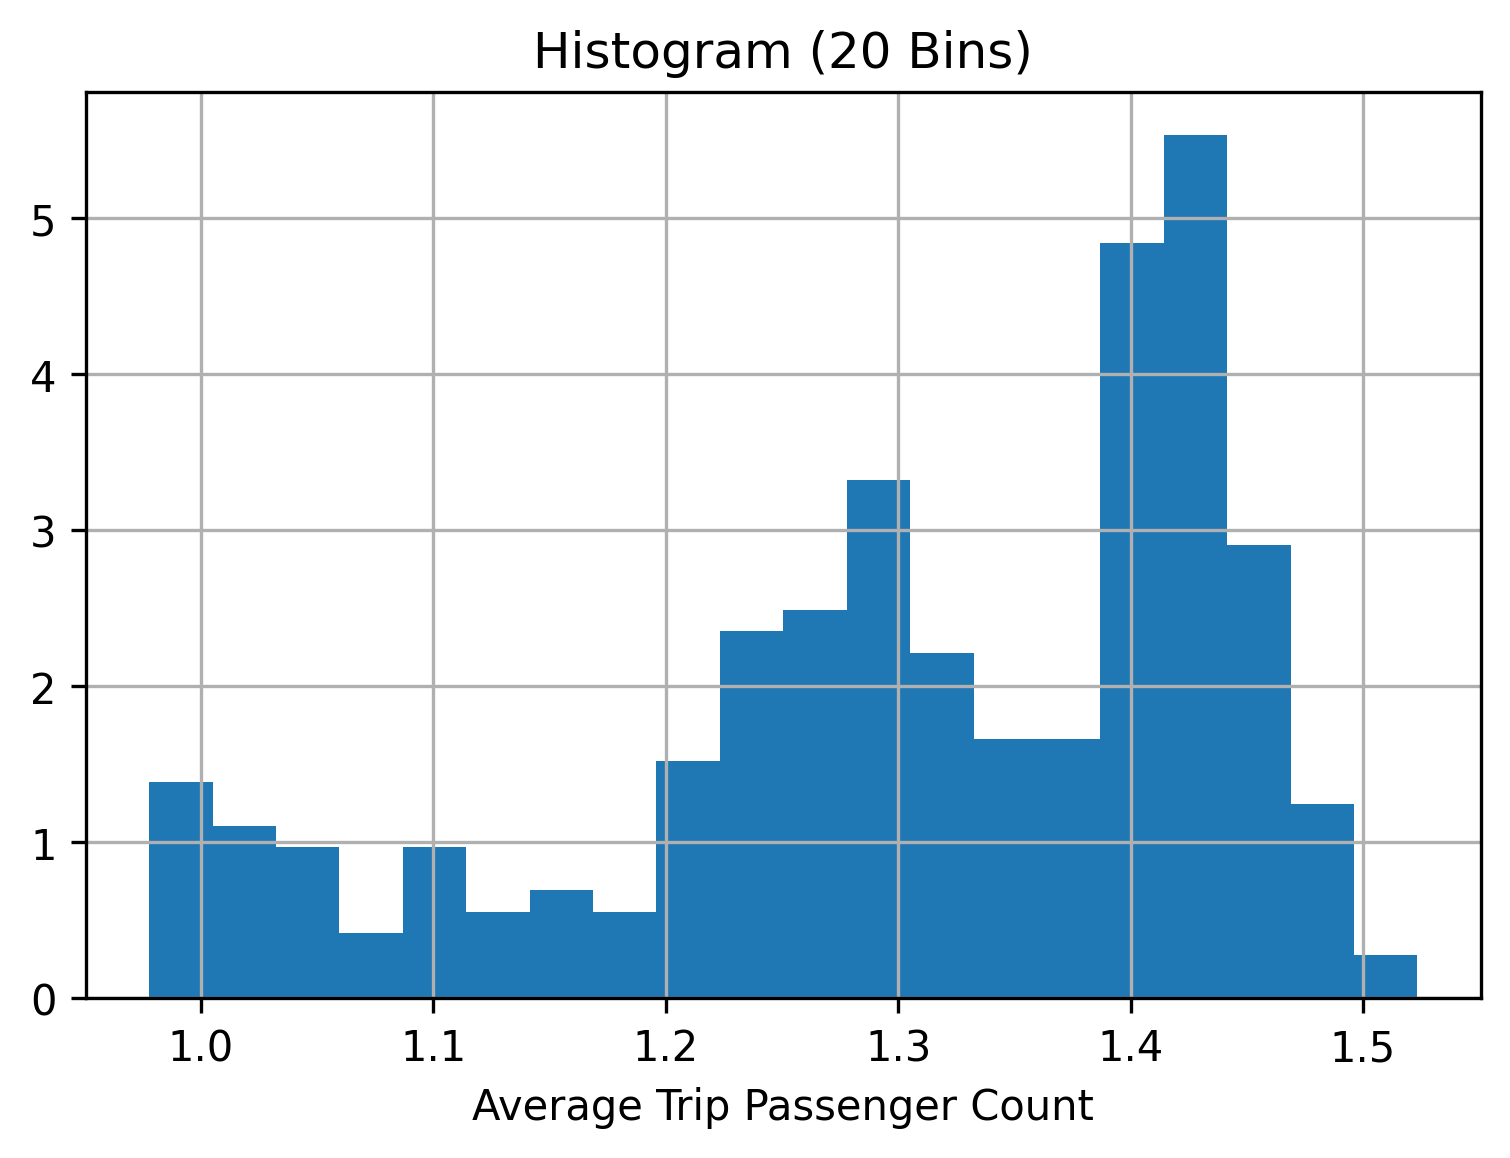
\includegraphics[width=0.38\textwidth]{../plots/histogram-Average Trip Passenger Count-20-bins.png}
    % this ensures your figures are centered where possible
    \centering
    \caption{Probability density histogram of average trip distance (left) and average trip passenger count (right) over Timeline 2.} % refer to this image as (Figure 1)
    \label{fig:hists}
\end{figure}

The selected reliance measures have different properties and distributions.
While the passenger count represents a discrete measure, trip distance is measured on a continuous scale.
The weekly average trip distances have an overall average of 

\subsubsection{Modelling}

\textbf{Weekly Average Trip Distance:}
The weekly average trip distance is

% \begin{enumerate} 
%     \item Example for enumerated points
%     % use \item to create more points
% \end{enumerate}

% \begin{itemize} 
%     \item Example for dot points
%     \item[*] You can change dot points to any symbols by putting [SYMBOL].
%     \item[$\times$] Here's a fun example.
% \end{itemize} 
% \lipsum[4-5]
% Example code for figures:
% % the [h] ensures your figure is inline at the location and not displayed on some other page
% \begin{figure}[h]
%     % change the scale multiplier to make the figures smaller or larger
%     \includegraphics[width=0.35\textwidth]{example-image-a}
%     % this ensures your figures are centered where possible
%     \centering
%     \caption{Some caption} % refer to this image as (Figure 1)
% \end{figure}
% \lipsum[1-2]

% Example of a maths equation:
% \begin{equation}
%     Y = X\beta + \epsilon
% \end{equation}

% Example of an aligned equation (\& denotes the symbol to align):
% \begin{align*}
%     E[\mathbf{y}] &= X\beta + E[0] \\
%                   &= X\beta
% \end{align*}

% Example of an in-line equation $\epsilon \sim N(0, 1)$ \\

\section{Conclusions}

This report provides a brief, but thorough look at correlations to simple reliance statistics.


\section{Recommendations}
This has been a thorough, but brief look into correlations between viruses and reliance metrics.
The following are several paths on which further research in this area could begin:
\begin{itemize}
    \item As mentioned in the paper, aggregation of TLC data performs grouping by pickup location.
    This means the same analysis should also be performed on aggregation by dropoff location instead.
    It would be interesting to compare and contrast the resulting models generated with this different grouping.
    \item There is the obvious path of modelling demand in the form of trip rates with respect to viral case rates. 
    \item It may be beneficial to begin generating models of repeated trips between the same locations,
    which could suggest patterns of use.
    \item Another way in which the research could be deepened would be to select a subset of specific locations where trips going to/from are likely work-related. 
    This would provide a window into measuring the shift to working from home caused by viruses.
    \item It should also be considered that there are other taxi and transport datasets available.
    A long-term goal of further research could be to model the effects of viruses on different modes of transport.
    This could then be applied to improve on transport sectors where the correlations to case rates have a stronger apparent effect.
    \item Finally, the results generated in this report are far from conclusive or exhaustive.
    As data is collected over the years, more accurate models may be constructed. 
    While the focus may remain on modelling against COVID-19 and Influenza rates, 
    other viral statistics such as the prevalence of HIV/AIDS should also be considered for potential correlations.
\end{itemize}

\clearpage

% BEGIN REFERENCES SECTION
\printbibliography

\end{document}